%====================================================================
% 修論てんぷれ 
%
%       メモ
%               章(chapter)>節(section)>項(subsection)
%               2行空白をあけるためには…   \vspace{2\Cvs}
%
%====================================================================
\documentclass[a4j,12pt]{jreport}
\usepackage{graphicx}

%====[ テスト ] ====================================================
\newcommand{\figtb}[5]{ %引数 {日本語タイトル}{英語タイトル}{サイズ}{ファイル名}{ラベル名}
\begin{figure}[tb]
  \begin{center}
    \includegraphics[width=#3cm,clip]{figure/#4}
    \caption{#1}
    \label{fig:#5}
  \end{center}
\end{figure}}

%====[ プリアンプル ]================================================
%
% 不必要ならコメントアウトするとコンパイルが速くなる
%       パッケージの機能は「tex パッケージ名」で検索
%
\usepackage{subfigure}  % 図に(a)(b)(c)と記号を振れるパッケージ
\usepackage{amsfonts}   % \mathbb 4兄弟 (数式の太文字フォント/自然数Nとかで使う)
\usepackage{amsmath}    % \mathbb
\usepackage{amssymb}    % \mathbb
\usepackage{multirow}   %表のmaltirow
%\usepackage{bbm}               % \mathbb
%\usepackage{enumitem}  % 箇条書きのフォーマットを編集できる
%\usepackage{theorem}   % 補題/定理/定義 
%\usepackage{boites}    % 文章を枠で囲む
%\usepackage{cases}             % 場合分けした数式に式番号をつける
%\usepackage{mathrsfs}  % 花文字
%\usepackage{fancybox}  % verbatimを四角で囲む

%以下の2行はコメントアウトすると卒業できなくなる
\usepackage[HeaderWithUnderline]{shuronABS}     % アブストラクト
\usepackage{penguin}    % ページレイアウト設定

%====[ 表紙 ]========================================================
\begin{document}
\addtitlepage           % タイトル
\tocpage                        % 目次

%====[ 本文 ]========================================================

\newcommand{\tensaku}[1]{#1}
%\newcommand{\tensaku}[1]{}

% vim: set tabstop=4 :
%**********************************************************
\chapter{はじめに}
\label{sec:intro}
%**********************************************************
\tensaku{\section{人流シミュレーションの背景と需要}}
駅や商業施設,イベント会場などのように人が多く集まる場所では,
利便性の向上や災害時の逃げ遅れ防止などの安全性の向上などの観点から
混雑や滞留の対策が重要である.


人が多く集まる場所




\tensaku{\section{人流シミュレーションの背景と需要}}
滞留などの対策が重要である\cite{taisaku1}\cite{taisaku2}.

感染シミュレーションもあるよ\cite{mas_pandemic}

人が多く集まるイベントなどの場所では,想定よりも多くの人が集まることで,
群集事故が発生する恐れがある.
群集事故は,人が将棋倒しのように倒れる群衆雪崩や〇〇である.
群衆事故を防止するには,急に狭くなる空間を作らないことや階段や出口を
広くするなどが有効である(参考文献).
%https://toyokeizai.net/articles/-/631584?page=3
人の滞留や避難時間の予測に人流シミュレーションが用いられている.
\cite{sim_jirei1}\cite{sim_jirei2}\cite{sim_jirei3}\cite{sim_jirei8}\cite{sim_jirei7}.

人流シミュレーションは,コンピュータ上で人を運動方程式に基づくエージェントとして
解析する手法である.
人流シミュレーションのなかでも歩行者の動きの再現には,
ネットワークモデルやフロアフィールドモデル,SocialForceModel(SFM)などが広く用いられている\cite{helbing_sfm}\cite{sfm_ntt}.
\tensaku{\section{ネットワークモデル}}
ネットワークモデルは,〇〇である.
ネットワークモデルは,災害時における都市部の避難シミュレーションなどの
大域的な解析を高速に解析が可能であるが,群集事故の防止に必要な滞留などの
解析ができないことが報告されている.
このため,建物内などの滞留の解析には,フロアフィールドモデルやSFMが
よく用いられている.(参考文献)
\tensaku{\section{フロアフィールドモデル}}
フロアフィールドモデルは,~~の手法である\cite{floa_field1}\cite{floa_field2}.
群集雪崩などの解析にも用いられる\cite{floa_field3}.



フロアフィールドモデルを用いた避難シミュレーションは,一つの格子が
人の大きさに制約されるため,出口付近で見られる滞留(アーチ現象)の
解析精度が低いことが報告されいている.
高い解析精度が必要な場合は,解析領域を二次元の連続座標として解析する
SFMがよく用いられている(参考文献).
\tensaku{\section{ソーシャルフォースモデル}}
SFMは,社会心理学的な要素と物理学的な要素で成り立つ運動方程式をエージェントごとに計算する
ことで,人流の動きを再現する手法である\cite{helbing_sfm}.
SFMの運動方程式は,目的地に向かう力,周囲のエージェントを避ける力,障害物を避ける力の
合力を算出し,エージェントの速度や進行方向を計算する.
SFMの運動方程式の計算は,エージェントや障害物の数の増加に応じて解析時間が
膨大になることから高速化が求められている.


SFMの避難シミュレーションの文献\cite{sfm_hinan1}\cite{sfm_hinan2}\cite{sfm_hinan3}.

人流シミュレーションのなかでも,歩行者の動きの再現には,視野やグループ特性などの
パラメータを追加できるSocial Force Model(SFM)が広く用いられている
\cite{helbing_sfm},\cite{sfm_ntt},\cite{sfm_para1},\cite{intro_gunshu}
.

視野パラメータを使っている文献\cite{siya_ex2}\cite{siya_ex3}\cite{siya_ex4}\cite{siya_ex5}\cite{siya_ex6}\cite{siya_ex7}


%\cite{siya_ex5},\cite{siya_ex4},\cite{siya_ex6}.


\tensaku{\section{SFMの高速化技法}}
一般的なSFMの高速化技法として,単位時間あたりの計算回数の増加や,
モデルの単純化,
エージェント間距離の計算回数の削減が行われている.
SFMの単位時間あたりの計算回数の増加には,GPU(Graphics Processing Unit)や
MPI(Message Passing Interface)を用いた並列処理を用いることが一般的である
\cite{seru_sfm1}\cite{seru_sfm2}
\cite{sfm_gpu1}\cite{sfm_gpu2}\cite{sfm_gpu3}\cite{sfm_gpu4}.
\cite{mpi1}\cite{mpi2}
SFMは,エージェントごとの運動方程式の計算に並列性があるため,
高い並列性を得ることができる(参考文献[GPUやMPIを使っている論文]).
GPUを用いた並列化手法は,エージェントごとに必要な進行方向の計算を
複数スレッドで並列に計算する.
モデルの単純化は,計算負荷が高いSFMの運動方程式の計算を一次元に簡易化
することで,解析時間を削減する手法である(参考文献[一次元化モデル]).
SFMの一次元化手法は,許容できる範囲の誤差で避難完了時間を解析できるが,
出口付近などの滞留の再現度が低いことが報告されている
(参考文献).
エージェント間距離の計算回数の削減には,影響半径の設定や,
セル分割法が提案されている\cite{cell1}\cite{cell2}.
影響半径は,エージェント間の距離が大きくなるほど相互作用力が
大きくなることを利用し,相互作用力が0に近似可能な距離を設定する.
影響半径を設定することで,影響半径外のエージェントに対する
相互作用力が計算不要となる\cite{eikyo_space}.
セル分割法は,解析領域を格子状のセルに分割し,周囲のエージェント
に対する影響範囲内外の判定をセル単位で実行する手法である.
影響範囲内外の判定には,エージェント間距離の計算が必要となるため
複数のエージェントに対する判定処理をまとめて実行することで,
エージェント間距離の計算回数を削減する.

リンクリスト法\cite{cell_book1}\cite{cell_book}\cite{cellrenketu}
ハッシュ法\cite{hash}

視野片寄の文献\cite{katayose}

%要検討(自分の手法をここに書くかどうか)
\tensaku{\section{提案手法}}
\if 0
壁多い
⇒障害物の計算が多い

壁の特徴
a

そこで!!
~~する
\fi
建物内の避難時におけるシミュレーションは,壁や机といった障害物が多く,
障害物を避ける力の計算回数が多い傾向がある.
障害物を避ける力は,エージェントの座標と障害物の座標を用いて計算する.
壁や机などの障害物は,解析中に座標が変化しない特徴がある.
そこで,本論文は,解析領域を格子に分割し,格子領域ごとにあらかじめ
進行方向を計算し,メモリ領域に保存することで,解析中の進行方向の
計算回数を削減する.


\if 0
%過去
商業施設やイベント会場などの人が多く集まる場所では,
災害時の逃げ遅れの観点から
人の滞留の対策が重要であり\cite{taisaku1},\cite{taisaku2},
人の滞留や避難時間の予測に人流シミュレーションが用いられている
\cite{sim_jirei1},\cite{sim_jirei2},\cite{sim_jirei3},\cite{sim_jirei8}.
人流シミュレーションは,コンピュータ上で人を運動方程式に基づくエージェントとして
解析する手法である.
人流シミュレーションのなかでも,歩行者の動きの再現には,視野やグループ特性などの
パラメータを追加できるSocial Force Model(SFM)が広く用いられている
\cite{helbing_sfm},\cite{sfm_ntt},\cite{sfm_para1},\cite{intro_gunshu}.
%\cite{siya_ex5},\cite{siya_ex4},\cite{siya_ex6}.

%\subsection{ソーシャルフォースモデル}
SFMは,社会心理学的な要素と物理学的な要素で成り立つ運動方程式をエージェントごとに計算する
ことで,人流の動きを再現する手法である.
SFMの運動方程式は,目的地に向かう力,周囲のエージェントを避ける力,障害物を避ける力の
合力を算出し,エージェントの速度や進行方向を計算する.
SFMの運動方程式の計算は,時間ステップごとに全てのエージェントに対して計算するため,
エージェント数の増加するほど,解析時間が膨大になることから高速化が求められている.

%\subsection{ソーシャルフォースモデルの高速化技法}
SFMでは,解析時間の高速化をするために,
モデルの1次元化や
エージェント間距離の計算回数の削減が行われている.
%
%\subsubsection{モデルの単純化}
SFMは,エージェントの動きを1次元に簡略化することで,
計算負荷を削減できる
\cite{1ji_sfm1},\cite{1ji_sfm2}.
SFMの1次元化は,避難人数や避難時間などの解析に対して許容できる
範囲の誤差で高速に解析ができるが,滞留の様子や人の密度などの解析ができないことが
報告されている\cite{1ji_sfm1}.
%
%\subsubsection{エージェント間距離の計算回数の削減}
エージェントを避ける力の計算には,エージェント間の距離が必要である.
エージェント間距離の計算回数の削減には,影響半径の設定や,
セル分割法が広く用いられる
\cite{seru_sfm1},\cite{seru_sfm2},\cite{katayose}.
影響半径の設定は,周囲のエージェントを避ける力や障害物を避ける力の
影響力が遠くなるほど0に近づく特性を利用し,影響半径外から受ける力を0に
近似することで,エージェント間距離の計算回数を減らす手法である.
セル分割法は,解析領域を格子状のセルに分割し,
周囲のエージェントに対する影響範囲内外の判定をセル単位で実行する方法である.
影響範囲内外の判定には,エージェント間距離の計算が必要となるため,
セル単位で判定することで,エージェント間距離の計算回数を削減する.
%\subsection{提案手法}
避難時を再現する人流シミュレーションは,机や壁などの障害物が多いため,
障害物を避ける力の計算回数が多い傾向がある.
机や壁などの固定された物である障害物や目的地は,解析中に座標が変化しないという特徴があり,
目的地まで向かう力を計算するために必要なエージェントから目的地までのベクトルは,
エージェントの座標に応じて決定するという特徴がある.
そこで,本論文では,解析前に目的地までの方向と障害物を避ける力の計算をあらかじめ計算し,
メモリに格納することで,
解析中の障害物を避ける力の計算と目的地までのベクトルの計算回数を削減する手法を提案する.
提案手法は,障害物が固定である特徴と目的地までのベクトルがエージェントの座標に応じて決まる特徴に
着目し,解析領域を格子状に分割した領域ごとに進行方向をあらかじめ計算する.
%}}}
\fi 




以下の章では,まず,ページフォーマットを示すために,
第\ref{sec:background}章で「あああああ」を述べる.
次に,第\ref{sec:survey}章で,本スタイルファイルで定義したコマンドについて述べる.
最後に,題\ref{sec:discuss}章でまとめる.


%***** END ************************************************

%------------------------------------------------------------------
% 注意点
%------------------------------------------------------------------
% 「はじめに」は,文章の導入部です.
% 論理構成を意識し,3年生にも分かるような説明を心がけましょう.
% 
% 研究背景について述べる必要があるため,サーベイの内容を多く書くことになります.
% 参考文献を多く挙げるようにしましょう.
% 
%
% ※当研究室では2ページ以上書かかないと前川先生にOKがもらえません. 
% 
% 
% 
% 一般的には以下のような構成になると思います.
% [1段落目]
% 背景&需要について書きます.
% この研究によって誰が喜ぶのかが分かるように書きましょう.
% [2段落目]
% 従来手法とその問題点について書きます.
% 1段落目の需要があるのに,誰も研究していないなんてことはありえません.
% [3段落目\UTF{FF5E}]
% 従来手法に対する改良手法について書きます.
% 従来手法の問題点が明らかになっているのに,誰も解決しようとしていないなんてありえません.
% 場合によっては手法ごとに段落を分けて書くこともあると思います.
% 研究に直接的に関係のないサーベイ内容も,ここにならがんがん書きましょう.
% [4段落目]
% 従来の改善方法で十分でしょうか?
% 不十分ならどのような手法が必要でしょうか?提案してください.
% [5段落目]
% 提案手法の手順や特徴を述べます.
% [6段落目]
% 「以降の章では\UTF{FF5E}」の文を書きます.
% 箇条書きになりやすいので,注意しましょう.
% 
%------------------------------------------------------------------

% vim: set tabstop=4 :
%**********************************************************
\chapter{人流シミュレーション}
%\chapter{本来なら問題定義や背景的な何かを書く}
\label{sec:background}
%**********************************************************

%1ブロックが10×30文字です
ああああああああああああああああああああああああああああああ
ああああああああああああああああああああああああああああああ
ああああああああああああああああああああああああああああああ
ああああああああああああああああああああああああああああああ
ああああああああああああああああああああああああああああああ
ああああああああああああああああああああああああああああああ
ああああああああああああああああああああああああああああああ
ああああああああああああああああああああああああああああああ
ああああああああああああああああああああああああああああああ
ああああああああああああああああああああああああああああああ
%
ああああああああああああああああああああああああああああああ
ああああああああああああああああああああああああああああああ
ああああああああああああああああああああああああああああああ
ああああああああああああああああああああああああああああああ
ああああああああああああああああああああああああああああああ
ああああああああああああああああああああああああああああああ
ああああああああああああああああああああああああああああああ
ああああああああああああああああああああああああああああああ
ああああああああああああああああああああああああああああああ
ああああああああああああああああああああああああああああああ
%
Penguin
ああああああああああああああああああああああああああああああ
ああああああああああああああああああああああああああああああ
ああああああああああああああああああああああああああああああ
ああああああああああああああああああああああああああああああ
ああああああああああああああああああああああああああああああ
ああああああああああああああああああああああああああああああ
ああああああああああああああああああああああああああああああ
ああああああああああああああああああああああああああああああ
ああああああああああああああああああああああああああああああ
ああああああああああああああああああああああああああああああ
%
ああああああああああああああああああああああああああああああ
ああああああああああああああああああああああああああああああ
ああああああああああああああああああああああああああああああ
ああああああああああああああああああああああああああああああ
ああああああああああああああああああああああああああああああ
ああああああああああああああああああああああああああああああ
ああああああああああああああああああああああああああああああ
ああああああああああああああああああああああああああああああ
ああああああああああああああああああああああああああああああ
ああああああああああああああああああああああああああああああ
%
ああああああああああああああああああああああああああああああ
ああああああああああああああああああああああああああああああ
ああああああああああああああああああああああああああああああ
ああああああああああああああああああああああああああああああ
ああああああああああああああああああああああああああああああ
ああああああああああああああああああああああああああああああ
ああああああああああああああああああああああああああああああ
ああああああああああああああああああああああああああああああ
ああああああああああああああああああああああああああああああ
ああああああああああああああああああああああああああああああ
ああああああああああああああああああああああああああああああ
%
ああああああああああああああああああああああああああああああ
ああああああああああああああああああああああああああああああ
ああああああああああああああああああああああああああああああ
ああああああああああああああああああああああああああああああ
ああああああああああああああああああああああああああああああ
ああああああああああああああああああああああああああああああ
ああああああああああああああああああああああああああああああ
ああああああああああああああああああああああああああああああ
ああああああああああああああああああああああああああああああ
%
ああああああああああああああああああああああああああああああ
ああああああああああああああああああああああああああああああ
ああああああああああああああああああああああああああああああ
ああああああああああああああああああああああああああああああ
ああああああああああああああああああああああああああああああ
ああああああああああああああああああああああああああああああ
ああああああああああああああああああああああああああああああ
ああああああああああああああああああああああああああああああ
ああああああああああああああああああああああああああああああ
ああああああああああああああああああああああああああああああ
%
ああああああああああああああああああああああああああああああ
ああああああああああああああああああああああああああああああ
ああああああああああああああああああああああああああああああ
ああああああああああああああああああああああああああああああ
ああああああああああああああああああああああああああああああ
あああああああああああああああああああああ
あああああああああああああああああああああ
%
%\chapter{背景(1671文字)}

%***** END ************************************************

% vim: set tabstop=4 foldmethod=marker foldlevel=0 :
%**********************************************************
%\chapter{一般的にはサーベイ内容とかを書く}
\chapter{人流シミュレーションの高速化}
\label{sec:survey}
%**********************************************************
SFMを用いた人流シミュレーションは,解析人数が多くなるほど計算負荷が
膨大になるため,解析に時間がかかる.
SFMの解析時間を削減するために,モデルの単純化(参考文献)や
エージェント間距離の計算回数削減手法(参考文献),
単位時間あたりの計算回数の増加手法 (参考文献),
経路選択時の判定回数の削減手法(参考文献)などが提案されている.
本章では,SFMの各高速化手法について述べる.

\section{モデルの簡易化}

\subsection{一次元化}
モデルの一次元化による高速化手法(一次元歩行者モデル)は,SFMの計算負荷を削減するために,
エージェント同士の受ける力や壁や机などの障害物を避ける力の計算を
簡略化し,解析する(参考文献).
図\ref{fig:1jigen_ex}に一次元歩行者モデルの例を示す.
図\ref{fig:1jigen_ex}中の△△は〜〜である.
図\ref{fig:1jigen_ex}



〜〜できるため,解析時間を削減できる.
一方で,本手法はエージェントの動きを二次元から一次元に簡易化していることから,
図\ref{fig:atigenshou}に示すようなアーチ現象を再現することができない.

\begin{figure}[hbtp]
 \begin{center}
  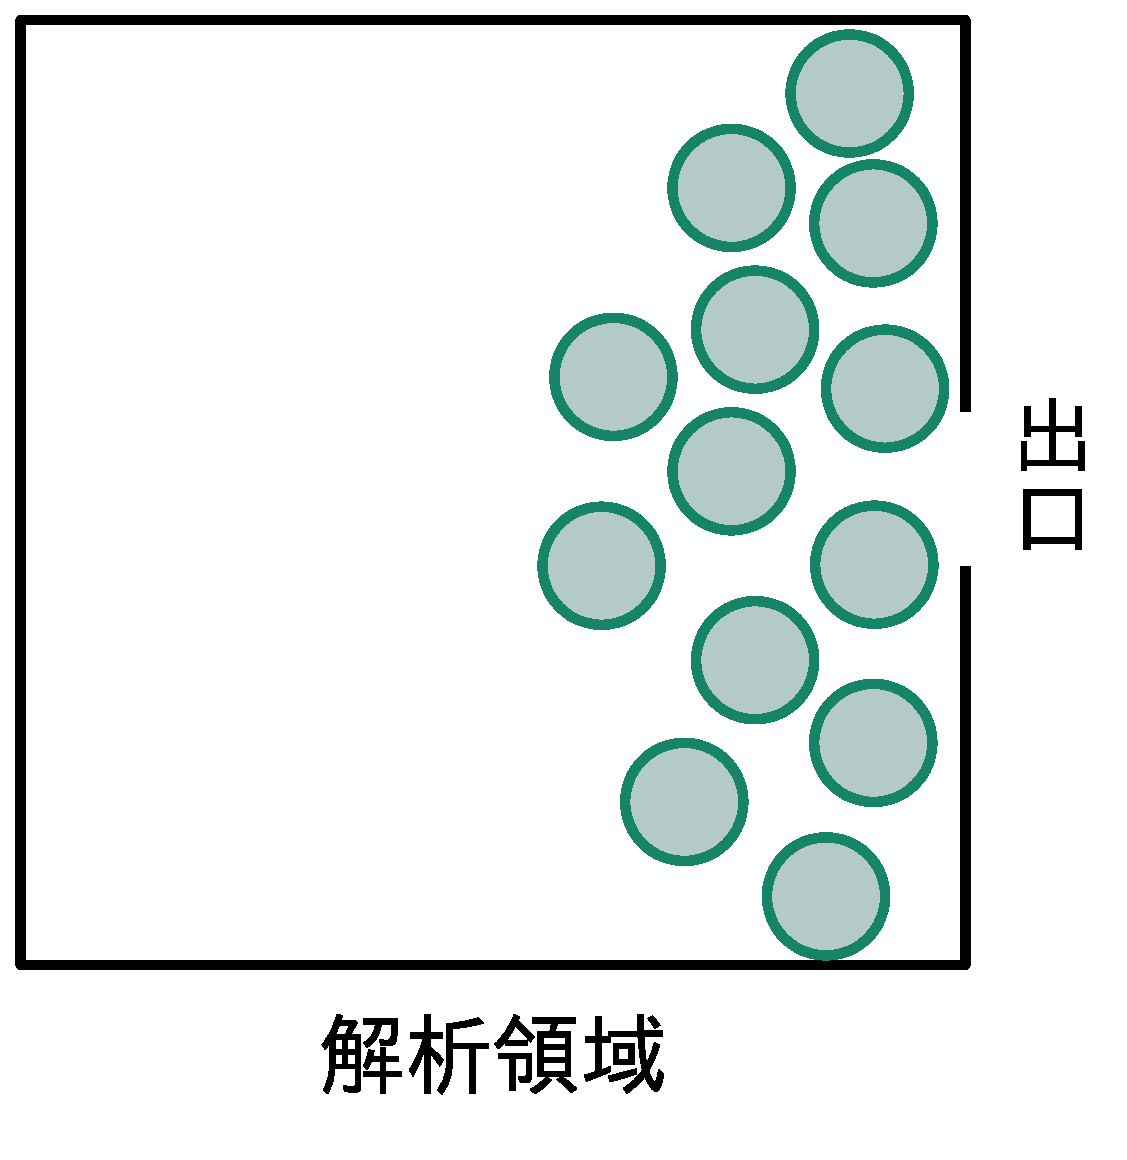
\includegraphics[width=5cm,clip]{figure/atigenshou.eps}
  \caption{アーチ現象の例}
  \label{fig:atigenshou}
 \end{center}
\end{figure}


\subsection{~~}

\section{エージェント間の距離の計算回数削減}
SFMは,解析人数が増加するほど周囲のエージェントから受ける力の計算に
必要なエージェント間距離$d_{ij}$の計算も増加する.
このため,SFMは,エージェント間距離$d_{ij}$の計算回数の削減による
解析時間の削減が行なわれている.
エージェント間距離の計算回数削減手法にセル分割法や視野パラメータを用いた
削減手法が提案されている.

\subsection{セル分割法}
セル分割法は,


\subsection{視野パラメータを用いた削減手法}

\section{単位時間あたりの計算回数}

\subsection{エージェントごとの並列性を用いた手法}

\subsection{解析領域ごとの並列性を用いた手法}

\section{経路選択時の判定回数削減}

\subsection{経路選択の単純化}

\subsection{経路選択手法の~~}




スタイルファイルの使い方について少し述べます.
普通に利用する分には,
拡張子が.texファイルのみを編集するだけで事が足りるように設計しました.
ただし,拡張子が.styファイルの書き換えは制限しません.自由に改変してください.


%----------------------------------------------------------
\section{abstract.tex}
%----------------------------------------------------------
abstract.texを書き換えると表紙およびアブストラクトを生成します.
abstract.tex内のコメントにしたがって書き換えを行ってください.
卒論にはアブストラクトが不要です.
修士のみアブストラクトを作成してください.

また,アブストラクトの設定はshuronABS.styに書いてあります.
表紙の設定はpenguin.styに書いてあります.
困ったときはこれらのファイルを変更してください.

%----------------------------------------------------------
\section{簡単コマンド}
%----------------------------------------------------------

penguin.styの294行目以降には, ショートカットコマンドを記述しました.
気が向いたら使ってやってください.
あくまでショートカットコマンドなので,
penguin.styのコマンドを使わなくても同じ機能を実現することができます.

\begin{itemize}
\item $\setminus$owata
\item $\setminus$ol\{ 数式 \}
\item $\setminus$fig\{ タイトル\}\{ ファイル名\}\{ 図の横幅[cm]\}
\item $\setminus$doublefig\{ タイトル1\}\{ ファイル名1\}\{ 図の横幅1[cm]\}\{ 図と図の間隔[cm]\}\{ title\_2\}\{ file\_name2\}\{ size\_2[cm]\}
\item $\setminus$figref\{ fig:ラベル\}
\item $\setminus$tabref\{ tb:ラベル\}
\end{itemize}


\figref{fig:ulysses16}に,$\setminus$figコマンドを用いて図を貼る例を示します.
\figref{fig:ulysses16}は,
$\setminus$fig\{適当な図を張ってみた\}\{ulysses16\}\{5\}で貼り付けています.
\figref{fig:ulysses16}では,図の横幅が5cmになるように大きさ指定をしています.


また,\figref{fig:test1}と\figref{fig:test2}は,
$\setminus$doublefigコマンドを用いて図を並べた例です.
これらの図は,$\setminus$doublefig\{横並び(左)\}\{test1\}\{2.5\}\{0.5\}\{横並び(右)\}\{test2\}\{2.5\}
で貼り付けています.
$\setminus$doublefigコマンドは,図のタイトル高さを自動調節する機能を持っていません.
このため,タイトルの高さは手動で調節してください.

\fig{適当な図を張ってみた}{ulysses16}{5}
\doublefig{横並び(左)}{test1}{2.5}{0.5}{横並び(右)}{test2}{2.5}

図を入れる時には,段落と段落の間に入れてください.
決して文の途中に図が入ることがあってはいけません.
もし,図を参照しているページと図のページが離れてしまった場合は,
段落の長さが適切でない可能性があります.
フォーマットを変えるのではなく,本文の構成を見直しましょう.


%----------------------------------------------------------
\section{参考文献}
\label{sec:bib}
%----------------------------------------------------------
参考文献を参照する文の例です\cite{1983_Ibaraki}.
参考文献の書き方には,bibファイルを使う方法と使わない方法の2通りがあります.
好きな方を選択し,makefileとmain.texを書き換えてください.

\subsection{bibファイルを使う場合}
main.texとmakefileの書き換えは必要ありません.
bibfile.bibに参考文献の記述例があります.
ciniiやIEEEなどでは文献のbibtex情報が用意されているので,
そのファイルをコピペして使えるのが強みです.
また,本方式を使うと,人力で参考文献情報をソートする必要が無いのでありがたいです.
ただし,参考文献が1つも参照されていないとエラーが生じる模様です\cite{test1}.

以下にFAQを載せておきます.
\begin{itemize}
        \item   {\bf bibファイルって何?bibtexって何?}\\
        使い方はgoogle先生に聞いてください.
        \item   {\bf 参考文献情報を書き換えてもコンパイル結果に反映されない}\\
        main.bblファイルを消去してから再コンパイルしてください.
        \item   {\bf 参考文献スタイルを変更したい}\\
        参考文献のフォーマットを決めるファイルは,sty/ipsjunsrt.bstです.
        本ファイルは,情報処理学会のスタイルファイルです.
        \item   {\bf 名字が1文字の人の表示がおかしい}\\
        情報処理学会フォーマットの仕様です.論文提出直前にbblファイルを直接編集してください.
        \item   {\bf bibファイルでエラーが出る}\\
        大抵の場合はカンマ忘れが原因です.次点で参照タグ名の重複かな?
\end{itemize}



\subsection{bibファイルを使わない場合}
自力でthebibliographyの中身を書くパターンです.
bibfile.texに記述例があります.
記述した通りに表示されるため,直感的には分かりやすいです.
ただし,人力での作業量が多くなるので,この方式を使う場合は頑張ってください.

本方式を用いる場合は,以下のファイルの書き換えが必要です.

\begin{itemize}
        \item {\bf main.tex\ }  61行目($\setminus$bibliography\{bibfile\})をコメントアウトし,
                                                62行目($\setminus$input\{bibfile\})のコメントアウトをはずしてください
        \item {\bf makefile\ }  $\#$記号でコメントアウトしてください
        \item {\bf bibfile.tex\ }       ここに参考文献を書いてください.
                                                参考文献は,本文中での参照順番に手動で並び替えが必要です.
\end{itemize}

%***** END ************************************************

% vim: set tabstop=4 :
%**********************************************************
%\chapter{提案手法にあたる章}
%\chapter{格子分割を用いた進行方向計算の削減手法}
\chapter{エージェント間距離の削減手法}
\label{sec:method}
%**********************************************************
SFMの運動方程式では,エージェント間距離が大きいほどエージェント間に働く相互作用力が小さくなる.
このため,SFMでは,影響半径$R_{c}$を用いてエージェント間距離の計算回数を削減するのが一般的である.
\figref{fig:sougo_hani}に,エージェント4の影響半径の例を示す.
\figref{fig:sougo_hani}中の〇はエージェントであり,
オレンジ色の点線で囲まれた領域がエージェント4の影響範囲である.
影響半径$R_{c}$は影響範囲の半径であり,
影響範囲外から受ける力を0とすることで,
運動方程式を計算する際に演算を省略することができる.
一方,視野を用いたSFMでは,視野範囲外の相互作用力を0とする.
\figref{fig:sougo_hani}の例で,エージェント4が図中矢印の方向に移動する際には,
エージェント4の視野は,図中の緑色の領域のように設定され,
視野$\subseteq$影響範囲のような関係となる.

SFMで用いられるエージェント間距離の計算回数削減手法は,
影響範囲が円形であることを前提としており,
影響範囲が視野のように扇形の場合を想定していない.
例えば,\figref{fig:sougo_hani}のエージェント配置では,
半径$R_{c}$内の白い領域に存在する5つのエージェントが視野外にあるにも関わらず,
これらのエージェントに対するエージェント間距離の計算が必要となる.
人の視野角$\theta$は$\pi$以下であるため,
視野を用いたSFMに一般的なSFMのエージェント間距離の計算回数削減手法を用いると,
影響範囲を円形に絞り込みをした上で,%視野形状に合わせた
扇形に絞り込みを行う操作が必要となる.
このため,視野範囲外となる半径$R_{c}$内のエージェントが多く存在するほど,
相互作用力を0として計算するエージェントに対するエージェント間距離の計算回数が増える.
そこで,本論文では,
視野形状である扇形に近似した領域を設定し,
近似領域外のエージェントに対するエージェント間距離の計算回数を削減することで,
視野を用いたSFMを高速化する.

提案手法では,近似領域の算出に必要な計算時間を最小限に抑えるために,
長方形で視野範囲を近似する.
これに合わせて,
視野範囲はエージェントの進行方向前方に存在するため,
エージェントの進行方向を長方形の辺数に合わせて上下左右の4パターンに分類し,
エージェントの進行方向に応じた近似領域を設定する.
エージェントの進行方向の分類方法によりシミュレーション時間が変化する可能性があるため,
本論文では,既存手法であるセル分割法を含む6パターン実装し,その有効性を評価する.
%パターン2~6は,パターン1のセル分割法で用いたセルを利用しており,
%各手法の影響範囲の設定条件は\tabref{tb:hantei_jouken}の通りである.
提案手法であるパターン2~6は,いずれの手法もパターン1のセル分割法の考え方を基にしており,
時間ステップごとに影響範囲の近似領域を設定した上で,
近似領域内で影響範囲内となるエージェントを相互作用力を計算する対象として設定する.
\tabref{tb:hantei_jouken}に,エージェントの進行方向を分類する条件を示す.
ただし,\tabref{tb:hantei_jouken}で条件に数式が2つ記述されているものは,
両条件を満たす必要があることを表す.
また,
\figref{fig:90do_hamideru}に,\figref{fig:sougo_hani}のエージェント4に対して
\tabref{tb:hantei_jouken}の各実装パターンが設定する視野範囲の近似領域を示す.

\figtb{影響範囲の例}{An example of the scope of influence.}{3.7}{20230614_hanni_ex.eps}{sougo_hani}

\figtb{エージェント4の実装パターンごとの近似領域の例}{The approximation region for each pattern of agent 4.}{8}{20231007_hanni.eps}{90do_hamideru}

\figtb{進行方向ごとの近似領域}{The approximation regions for each direction.}{7}{20220225_sentaku.eps}{sentaku}

\begin{table*}[tb]
\begin{center}
\caption{進行方向を分類する条件}
\label{tb:hantei_jouken}
\begin{tabular}{c|c|c|c|c}
\hline \hline
			& 右 & 左 & 上 & 下 \\ \hline
パターン2   & $\frac{1}{\sqrt{2}} < e_x \leq 1  $
		    & $ -1 \leq e_x < \frac{-1}{\sqrt{2}}$ 
		    & $ \frac{-1}{\sqrt{2}} < e_x < \frac{1}{\sqrt{2}} $ 
		    & $ \frac{-1}{2} < e_x < \frac{1}{2} $ \\
パターン3   & $\frac{-1}{2} < e_y < \frac{1}{2} $ 
		    & $\frac{-1}{2} < e_y < \frac{1}{2} $
            & $ \frac{1}{\sqrt{2}} < e_y \leq 1$
		    & $ -1 \leq e_y < \frac{-1}{\sqrt{2}} $ \\
\hline
\multirow{2}{*}{パターン4}   
			& $R_x \geq A_x$ & $R_x < A_x$ & $R_y \geq A_y$ & $R_y < A_y $ \\
	        &  $L_x \geq A_x$ & $L_x < A_x$ & $L_y \geq A_y$ & $L_y < A_y$ \\
\hline
\multirow{2}{*}{パターン5}   
 			& $R_x \geq x_1$ & $R_x < x_2$ & $R_y \geq y_1$ & $R_y < y_2 $ \\
			& $L_x \geq x_1$ & $L_x < x_2$ & $L_y \geq y_1$ & $L_y < y_2 $ \\
\hline
パターン6   & $ \cos(\frac{1}{2}\theta_{view}) \leq  e_y $ 
			& $ e_y \leq -\cos(\frac{1}{2}\theta_{view})$ 
			& $ \sin(\frac{1}{2}(\pi - \theta_{view})) \leq e_x $ 
			& $ e_x \leq \sin(\frac{1}{2}(\pi - \theta_{view}))  $ \\
\hline
\end{tabular}
\end{center}
\end{table*}

\section{パターン1(セル分割法)}
パターン1は,一般的なセル分割法\cite{cell1},\cite{cell2}によるエージェント間距離の計算回数削減を行う.
\figref{fig:90do_hamideru}では黄色の領域がセル分割法による近似領域を表す.
セル分割法は,\figref{fig:90do_hamideru}のように解析領域を格子状のセルに分割し,
影響半径$R_{c}$の円内に重なるセルを近似領域とする手法である.
本手法は,分割するセルのサイズを影響半径と同じ距離に設定することで,
近似領域をエージェントの近傍9セルに限定することができる.
本例では,エージェント4の近傍9セルは黄色のセルであり,
それ以外のセルに属するエージェント3,5,9に対するエージェント間距離の計算を削減できる.
なお,セル分割法は相互作用力を計算する範囲を円形で想定した手法であるため,
近似領域が正方形となることから,パターン1の実装では進行方向の推測は行わない.
また,本論文では,セル分割法のなかでもメモリ使用量を抑えることができると知られている
連結リスト法\cite{cell_book1},\cite{cell_renketu}を用いる.

\section{パターン2}
パターン2は,エージェントの進行方向を表す単位ベクトル$e_{i}$を参照することで,
パターン1の近似領域を視野範囲に近づける手法である.
本手法は,\tabref{tb:hantei_jouken}の条件に基づいて
単位ベクトル$e_{i}$が示す進行方向を上下左右を$\frac{1}{2}\pi$の均等な角度で分割し,
セル分割法の近似領域から\figref{fig:sentaku}のように進行方向の反対側にある3セルを除外する.
\figref{fig:90do_hamideru}の例では,エージェントの進行方向は右と判定され,
\figref{fig:sentaku}に示す右方向の青いセルを近似領域に設定する.
このため,白色のセルに存在するエージェントに対する距離計算を削減できる.
パターン2は,進行方向を必ず上下左右のいずれかに設定するため,
常に近似領域が6セルとなり,セル分割法の9セルに比べて近似領域の面積を$\frac{2}{3}$に削減できる.
一方で,\figref{fig:90do_hamideru}のように視野範囲全体が近似領域内に含まれる保障がないため,
本来相互作用力の計算が必要なエージェントに対する計算を削減し,誤差が発生する可能性がある.

\section{パターン3}
パターン3は,パターン2で発生する誤差を防ぐために,
近似領域外に視野範囲が存在しないかを判定する処理を追加し,
セル分割法と同じ精度を保つ手法である\cite{katayose}.
本手法は,パターン2の近似領域を導出したのち,
視野の座標$(L_x,L_y)$,$(R_x,R_y)$が
近似領域内のセルであればパターン2の近似領域を用いて相互作用力を計算し,
そうでなければパターン1の近似領域を用いて相互作用力を計算する.
\figref{fig:90do_hamideru}のエージェントは,
$L_{x}, L_{y}$がパターン2の近似領域の外にあるため,
パターン3ではパターン1と同様に近傍9セルを近似領域とする.
エージェントの座標は時間ステップごとに変化するため,
パターン3を用いると,進行方向が変化しないエージェントに対しても
すべての時間ステップでパターン1よりもエージェント間距離の計算を削減できるとは限らない.
一方で,パターン3は,パターン1のセル分割法と同じ精度のシミュレーション結果を得ることができる.

\section{パターン4}
パターン4は,視野の左右両端の座標$(L_x,L_y)$,$(R_x,R_y)$を用いて近似領域を設定する手法である.
視野範囲は進行方向の前方に存在するため,
視野の左右両端の座標はエージェント座標から見て必ず進行方向側となる.
この特性を利用し,パターン4では,\tabref{tb:hantei_jouken}のように,
エージェント座標$(A_x,A_y)$と視野座標$(R_x,R_y)$,$(L_x,L_y)$の
大小関係を用いて進行方向を判定する.
\figref{fig:90do_hamideru}の例では,$R_x \geq A_x$および$L_x \geq A_x$が成り立つため,
エージェントの進行方向は上と判定される.
進行方向が求まると,近傍9セルから進行方向反対側の3セルを除外した6セルを近似領域とする.
\tabref{tb:hantei_jouken}のいずれの条件にも当てはまらない場合は,
パターン1(セル分割法)と同様に近傍9セルを近似領域とする.

\subsection{パターン5}
パターン5は,セル分割法のセル座標と視野範囲の左右両端の座標$(L_x,L_y)$,$(R_x,R_y)$を
用いて近似領域を設定する手法である.
本手法は,運動方程式を算出するエージェントが所属するセルの
左上座標$(x_1,y_2)$および右下座標$(x_2, y_1)$を用いて,
\figref{fig:sentaku}の4パターンの水色の領域内に視野が収まっているかを判定する.
\figref{fig:90do_hamideru}の例では,
$R_y \geq y_1$および$L_y \geq y_2$が成り立つため,進行方向は上と分類される.
本手法は,エージェントのセル上の位置に応じて進行方向を分類するため,
ベクトル$e_i$の表す進行方向が同じエージェントでも
エージェント座標に応じて異なる方向に分類される可能性がある.
本手法も\tabref{tb:hantei_jouken}のいずれの条件にも当てはまらない場合は,
パターン1(セル分割法)と同様に近傍9セルを近似領域とする.

\section{パターン6}
パターン6は,パターン2で設定した上下左右の角度範囲を,
シミュレーション誤差の出ない範囲で設定する手法である.
パターン6では,
\figref{fig:sentaku}中の水色の領域である近似領域内に視野範囲がすべて収まる進行方向を静的に計算し,
エージェントの進行方向を表すベクトル$e_i$の閾値を定める.
視野角を$\theta_{view}$とおくと,
エージェント座標がどの位置であっても上方向と判定される進行方向の角度は
$\frac{1}{2}(\pi - \theta_{view})$から$\frac{1}{2}(\pi + \theta_{view})$の間であり,
これを用いて進行方向ベクトル$e_{i} = (e_{x}, e_{y})$の範囲が
$\sin{(\frac{1}{2}(\pi - \theta_{view}))} \leq e_{x}$という条件を設定できる.
パターン6は,パターン3~6のように視野座標$(R_x,R_y)$および$(L_x,L_y)$を算出する必要がないため,
他の分類条件よりも高速に進行方向を分類することができる.
一方で,進行方向が特定の方向である場合は,
エージェント座標に関係なくパターン1(セル分割法)と同じ近似領域を設定するため,
エージェント間距離の計算回数は,パターン1に次いで多くなると考えられる.

%***** END ************************************************

% vim: set tabstop=4 :
%**********************************************************
%\chapter{提案手法にあたる章}
%\chapter{格子分割を用いた進行方向計算の削減手法}
\chapter{格子分割による進行方向ベクトル計算の削減手法}
\label{sec:method}
%**********************************************************
SFMの運動方程式は,エージェントの位置が変わるたびに,
目的地までのベクトルを表す$e$や周囲のエージェントを避ける力$f_{ij}$,
障害物を避ける力$f_{iW}$の再計算が必要となる.
周囲のエージェントを避ける力$f_{ij}$の計算は,時間ステップごとにすべての
エージェントの位置が変化するため,解析中のみに計算が可能である.
一方,ベクトル$e$や障害物を避ける力$f_{iW}$は,エージェントの位置に
応じて決定し,壁や机などの障害物の座標が固定であることから,解析前に計算が可能である.

そこで,本論文では,格子状に分割した領域ごとにベクトル$e$と障害物を避ける力$f_{iW}$を
あらかじめ計算することで,解析中の進行方向の再計算を削減する.

\section{格子分割を用いた進行方向計算手法}
本手法は,解析領域を格子状に分割し,格子ごとに進行方向ベクトル$e$や
障害物を避ける力$f_{iW}$をあらかじめ計算する.
進行方向ベクトル$e$は,式\eqref{eq:sfm_siki1}に示すSFMの運動方程式から
$v_i^0(t)$が係数である.一方で,障害物から受ける力$f_{iW}$は,
式\eqref{eq:sfm_siki1}に示すように,式の第3項である.
このため,進行方向ベクトル$e$と障害物を避ける力$f_{iW}$は,
別々の配列に格納する必要がある.
\figref{fig:5_teian_flow1}に格子分割を用いた
進行方向ベクトル計算の削減手法のフローチャートを示す.
\figref{fig:5_teian_flow1}中の前処理は,提案手法に必要である格子ごとの進行方向や
壁を避ける力を算出する.
\figref{fig:5_teian_flow1}中の運動方程式を用いた計算は,
エージェントの進行方向を計算する処理であり,
エージェントの進行方向ベクトル$e$や
障害物を避ける力$f_{iW}$を前処理で算出した値を参照する.

\figtb{提案手法の解析全体のフローチャート}{}{4.5}{5_teian_flow1.eps}{5_teian_flow1}

%\subsection{格子分割を用いた進行方向ベクトル$e$の計算方法}
\subsection{格子ごとの進行方向ベクトル$e$の計算方法}
進行方向ベクトル$e$は,目的地に進むベクトルであり,エージェントの座標から
目的地の座標までのベクトルである.
このため,ベクトル$e$は解析領域を格子状に分割した領域ごとの中心座標から
目的地の座標までのベクトルを計算することで,解析前に計算が可能となる.
\figref{fig:grid_ex1}に格子分割した進行方向の例を示す.
%
\figtb{提案する格子分割の例}{}{9}{ex1.eps}{grid_ex1}
%
\figref{fig:grid_ex1}中の○はエージェントであり,エージェントA,Bが1つの目的地に向かう
様子である.
図中のエージェントBは,エージェントAの位置に移動したとき,エージェントAと同じ進行方向に
なる.
このため,解析領域を分割し,格子ごとに進行方向を算出することで,解析中の
進行方向の再計算が削減できる.
目的地と障害物が含まれる格子は,エージェントが正しく目的地に進むようにするために,
0ベクトルを格納する.
0ベクトルが格納された格子中に存在するエージェントは,
改めて個別に進行方向ベクトル$e$を計算する.
格子ごとの進行方向は,格子の中心座標から目的地までのベクトル$e$を求め,配列に格納する.
目的地の他に経由地が複数存在する場合,進行方向は,経由地ごとに異なるため,経由地ごとに違う配列に格納する必要がある.
\figref{fig:ex2}に経由地が複数存在する例を示す.
\figref{fig:ex2}中の右図は経由地の進行方向,左図は目的地の進行方向,青色の矢印は経由地に進む進行方向,
青矢印は目的地の進行方向,0は進行方向を個別計算するための0ベクトル,オレンジ色の四角は机などの障害物を示す.
\figref{fig:ex2}のように,経由地と目的地の進行方向は,それぞれの座標が異なるため,ベクトル$e$も大きく異なることから,
それぞれ別の配列で保持する必要がある.
式\eqref{eq:route_youso_size}に進行方向ベクトル$e$を格納するための配列の要素数を算出する式を示す.
%
\begin{eqnarray}
 \mbox{進行方向の格子の要素数[個]} = 
 \big( \frac{\mbox{解析領域[m]}}{\mbox{格子サイズ[m]}} \big) ^ 2 \times  2 \times \mbox{経由地数[個]}
 \label{eq:route_youso_size}
\end{eqnarray}
%
式\eqref{eq:route_youso_size}のように,進行方向を格納する配列は,
解析領域の大きさや格子サイズの小ささ,経由地数の大きさに応じて
要素数が増加する.
また,進行方向を格納する配列の前処理にかかる時間は,
配列の要素数に応じて格子ごとの進行方向計算回数が増加するため,
配列の大きさに応じて増加する.

%\figtb{経由地がある配置の例}{}{3}{5_original_ex.eps}{5_origin}

%\figtb{経由地がある場合の進行方向の例}{}{7}{ex2.eps}{ex2}
\figtb{経由地がある場合の進行方向の例}{}{12}{5_e_vec_ex.eps}{ex2}
%\figtb{シミュレーション中の進行方向計算のフローチャート}{}{8.5}{5_e_flow.eps}{5_e_flow}

%\subsection{格子分割を用いた障害物を避ける力$F_{iW}$の計算方法}
\subsection{格子ごとの障害物を避ける力$F_{iW}$の計算方法}
障害物を避ける力$F_{iW}$は,エージェントの座標と障害物の座標に応じて変化する.
障害物は,机や壁などの固定された物であるため,座標が変化しない.
このため,障害物を避ける力$F_{iW}$は,解析領域を格子状に分割した領域ごとの
中心座標と障害物の座標から解析前にあらかじめ計算が可能となる.
\figref{fig:preparation_fiw}に格子分割した障害物を避ける力$F_{iW}$を示す.
\figref{fig:preparation_fiw}中の四角は解析領域を格子状に分割した格子,
黒点は格子の中心点,緑色の丸は格子の中心点からの影響範囲,オレンジ色の
丸は壁粒子,赤色の矢印は黒点の中心点が受ける障害物を避ける力$f_{iW}$である.
\figref{fig:preparation_fiw}の例は,黒点が存在する格子が受ける障害物を避ける力$f_{iW}$
を示しており,黒点の中心点から緑色の範囲に存在する壁粒子から力を受ける.
各格子は,\figref{fig:preparation_fiw}のように格子の中心点の座標を
用いて障害物を避ける力を計算する.
壁を避ける力$F_{iw}$を格納する配列は,
経由地が変わっても変化しないため,解析領域全体で一つとなる.
式\eqref{eq:fiw_youso_size}に障害物を避ける力$F_{iW}$を格納する配列の要素数を示す.
%
\begin{eqnarray}
 \mbox{障害物を避ける力を格納する格子の要素数[個]} =  \Big( \frac{\mbox{解析領域[m]}}{\mbox{格子サイズ[m]}} \Big) ^ 2 \times 2
 \label{eq:fiw_youso_size}
\end{eqnarray}
%
式\eqref{eq:fiw_youso_size}に示すように,障害物を避ける力を格納する配列の要素数は,
解析領域と格子サイズに応じて決まり,解析領域を格子サイズで割った値の二乗が配列の要素数となり,
障害物を避ける力$F_{iW}$がxとy方向に存在するため,要素を2倍した値が障害物を避ける力$F_{iW}$を
格納する配列の総要素数になる.
\figref{fig:5_teian_flow2}に格子分割を用いた進行方向の計算回数削減手法の前処理のフローチャート
を示す.
\figref{fig:5_teian_flow2}中の$F_{iW}$配列は障害物を避ける力$F_{iW}$を格納する配列,
進行方向配列は進行方向ベクトル$e$を格納する配列,
$F_{iW}$のxインデックスとyインデックスは$F_{iW}$配列に格納するためのインデックスであり,
すべての要素に値を格納するためのループである.
同様に,進行方向配列のxインデックスとyインデックスは進行方向ベクトル$e$を配列に格納するための
インデックスであり,すべての要素に値を格納するためのループである.
進行方向ベクトル$e$は,経由地ごとに異なるため,経由地数分のループが前処理に必要となる.

%障害物が含まれる格子と周辺の格子に0を入れることを書く.

\figtb{格子分割した障害物を避ける力$F_{iW}$の例}{}{10}{5_fiw_grid.eps}{preparation_fiw}

%\figtb{提案手法の前処理のフローチャート}{}{5}{5_teian_flow2.eps}{5_teian_flow2}

\begin{figure}[p]
 \begin{center}
  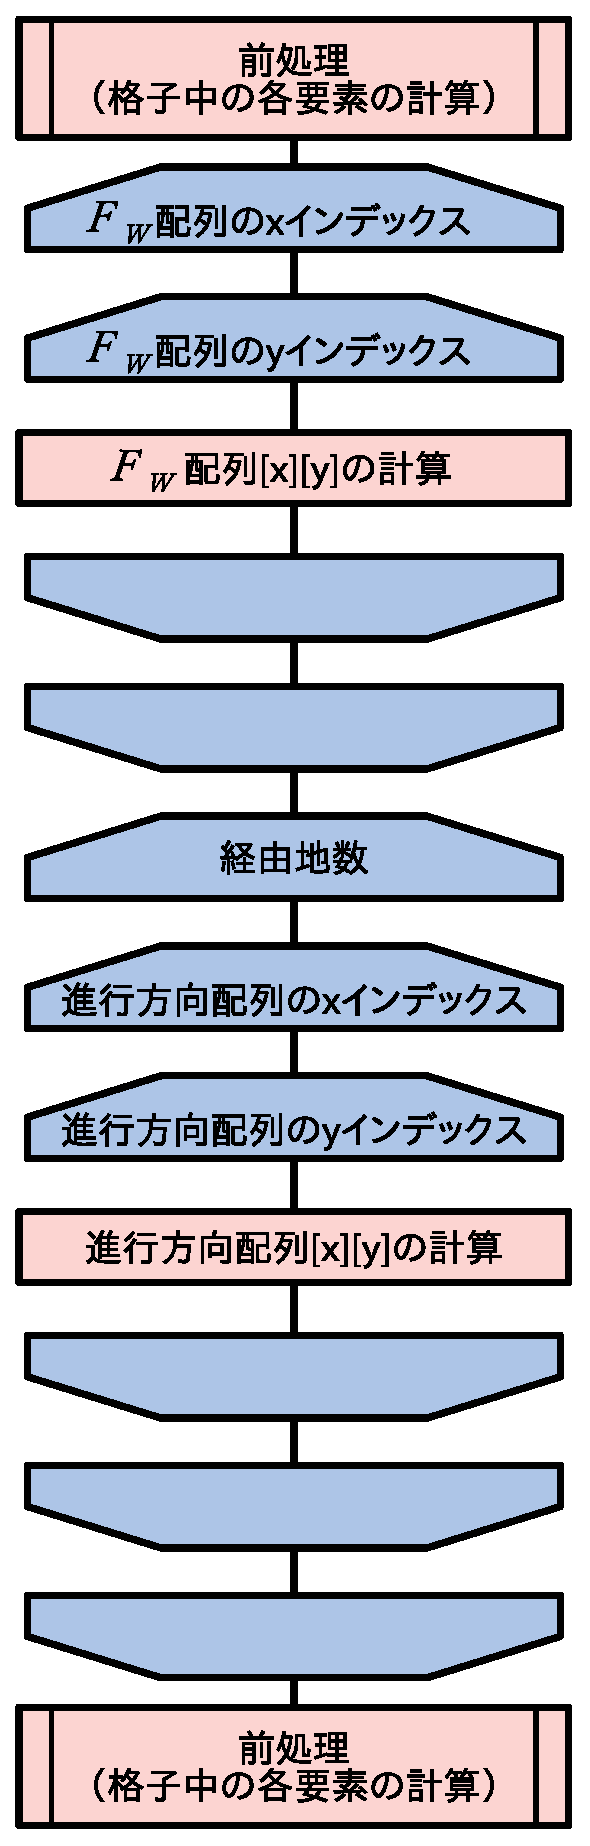
\includegraphics[width=4.5cm,clip]{figure/5_teian_flow2.eps}
  \caption{格子分割の前処理のフローチャート}
  \label{fig:5_teian_flow2}
 \end{center}
\end{figure}

\clearpage
\subsection{個別に進行方向を計算する格子の判定}
格子分割を用いた進行方向の計算回数削減手法は,精度の大幅な低下を防ぐために,
\figref{fig:ex2}のように目的地や障害物が含まれる格子とその周辺の格子に存在するエージェントを
個別に進行方向を計算するように設定する.
個別に進行方向する格子には,xとyの両方のベクトルに0が格納されているため,
解析中にエージェントが存在する格子に0ベクトルが格納されているか判定が必要となる.
\figref{fig:5_teian_flow2}に進行方向ベクトル$e$および障害物を避ける力$F_{iW}$の
解析中に個別計算するかどうかの判定のフローチャートを示す.
\figref{fig:5_teian_flow2}が示すフローチャートは,\figref{fig:5_teian_flow1}中の
解析中の運動方程式を用いた計算であり,エージェントの進行方向を求めるための計算である.
\figref{fig:5_teian_flow2}中の$F_{iW}$配列は障害物を避ける力$F_{iW}$を格納する配列,
進行方向配列は進行方向ベクトル$e$を格納する配列である.
\figref{fig:5_teian_flow2}に示すように,格子分割を用いた進行方向の計算回数削減手法は,
エージェントの座標から参照する配列の要素を求め,0ベクトルが格納されていない場合に
配列中の値を参照し,0ベクトルが格納されている場合に個別計算を行うことで解析中の
計算回数を削減する.

\figtb{提案手法の運動方程式計算のフローチャート}{}{9}{5_teian_flow3.eps}{5_teian_flow2}

\clearpage

\figtb{格子の進行方向とエージェントの進行方向で誤差が出る場合}{}{14}{5_kobetu_ex.eps}{5_kobetu_ex}
\figtb{近傍格子を個別計算の格子に設定する例}{}{8}{5_kobetu_ex1.eps}{5_kobetu_ex1}

\subsection{進行方向を個別に計算する格子の設定方法}
%\subsection{格子分割で発生する進行方向の誤差の抑止}
提案手法は,\figref{fig:ex2}のように格子ごとに中心座標から目的地や経由地までの進行方向を決定するため,
格子が大きくなるほど,エージェントの進行方向と格子の進行方向で誤差が生じる.
\figref{fig:5_kobetu_ex}にエージェントの進行方向と格子の進行方向で誤差が生じる例を示す.
\figref{fig:5_kobetu_ex}中の緑色の四角は解析領域の緑色の範囲を拡大したもの,
右側の目的地の進行方向は\figref{fig:grid_ex1}の目的地の進行方向,
赤色のひし形は目的地,赤色の矢印は進行方向,
白色の丸はエージェント,青色の矢印は既存手法で求めたエージェントの進行方向である.
\figref{fig:5_kobetu_ex}のように,提案手法を用いた進行方向は,格子ごとの中心座標から
目的地の座標に向かうベクトルを算出するため,図中の赤色の矢印のように表せる.
一方で,SFMの運動方程式を用いて計算したエージェントの進行方向は,
エージェントの座標から目的地の座標に向かうベクトルであるため,
図中の青色の矢印のように表せる.
\figref{fig:5_kobetu_ex}中のエージェントは,格子のサイズが大きいことや格子の端にいるために,
本来の進行方向と大きく誤差が生じることがわかる.
このため,本提案手法は,個別に進行方向を計算する格子の設定方法を目的地や障害物が存在する
格子と近傍の格子にすることで,エージェントの進行方向に大きな誤差が生じないように対策する.
\figref{fig:5_kobetu_ex1}に近傍の格子を個別計算の格子に設定する例を示す.
\figref{fig:5_kobetu_ex1}中の左側の四角は解析領域を示しており,
左の四角は格子ごとの目的地に向かう進行方向,格子内の0は,個別でエージェントの進行方向を計算する格子である.
\figref{fig:5_kobetu_ex1}のように,提案手法は,目的地や障害物を含む格子とその近傍の格子を
個別計算することで,\figref{fig:5_kobetu_ex}のようなエージェントの進行方向の誤差が発生することを防ぐ.



%\figtb{シミュレーション中の$f_{iW}$計算のフローチャート}{}{8.5}{5_e_flow.eps}{5_e_flow}


\clearpage
\section{評価}
SFMを用いた人流シミュレーションに対する
格子分割を用いた進行方向の計算回数削減手法の有効性を確認するために,
既存手法であるセル分割法と提案手法を用いて人流シミュレーション
評価環境は,\tabref{tb:result_env}に示すマシンである.
本評価では,\tabref{tb:result_para}に示すパラメータを用いて
SFMの運動方程式を計算する.
本評価では,避難時のシミュレーションを再現するために,
エージェント数よりも壁粒子が多い配置にエージェントを一方向に進むような解析を行う.
\figref{fig:5_initialconf}に本評価に用いるエージェントの初期配置を示す.
\figref{fig:5_initialconf}中の黄色の四角は障害物(壁),赤色のひし形は目的地,
緑色の四角はエージェントの初期配置位置である.
\figref{fig:5_initialconf}のエージェントは,緑色の範囲内から赤色の目的地まで
進むように設定する.本評価では,格子サイズごとの計算回数の削減率や,解析時間の
有効性を評価するために,\figref{fig:5_initialconf}に示す配置の壁の間隔や粒子数を変えた
複数パターンを用いる.
\figref{fig:haba2}と\figref{fig:haba5},\figref{fig:haba10},\figref{fig:haba20}に
評価で用いる\figref{fig:5_initialconf}のエージェントの初期配置の壁間隔を変えた配置を示す.
また,\figref{fig:haba2_2},\figref{fig:haba2_3}に通路幅2mのときの配置(\figref{fig:haba2})
の壁粒子をそれぞれ2倍,3倍にした配置を示す.
図中の黒丸は壁粒子,紫色の丸はエージェント,青色の丸は目的地である.
図に示す配置のエージェントは40人,壁粒子は592個,経由地は1個,
解析領域は$50m \times 50m$である.
また,壁粒子を変えた配置(\figref{fig:haba2_2},\figref{fig:haba2_3})の
壁粒子数は\tabref{tb:haba_atusa}に示す通りである.
図中のすべてのエージェントは,青色の丸が示す目的地に向かうように設定する.
測定する格子サイズは,解析領域の一辺(50m)を半分ずつ割った値を用いる.

\begin{table}[t]
  \begin{center}
    \caption{評価環境}
      \label{tb:result_env}
      \begin{tabular}{c|c}
      \hline \hline
      CPU              & Intel Xeon CPU E5-2667w v2 \\ \hline
      メモリ           & 32GB                       \\ \hline
      OS               & Linux 6.5.8               \\ \hline
      コンパイラ       & gcc 13.2.0                  \\ \hline
      最適化オプション & -O3                        \\ \hline
    \end{tabular}
  \end{center}
\end{table}

\begin{table}[t]
  \begin{center}
    \caption{測定条件}
    \label{tb:result_para}
    \begin{tabular}{c|c}
      \hline \hline
      $A_i$            & 2000N                              \\ \hline 
      $B_i$            & 0.08m                              \\ \hline 
      $k$              & $1.2 \times 10^5 kg s^{-2} $       \\ \hline 
      $\kappa$         & $2.4 \times 10^5 kg m^{-1} s^{-2}$ \\ \hline 
      $v_i^0$          & $1.4$m/s                           \\ \hline 
      $m_i$            & $80$kg                             \\ \hline 
      $\tau_i$         & 0.5                               \\ \hline 
      $r_i$            & $0.25$m                            \\ \hline 
      相互作用範囲     & $5$m                              \\ \hline 
    \end{tabular}
  \end{center}
\end{table}


\begin{table}
  \begin{center}
    \caption{壁の厚さを変えたときの初期配置のパラメータ}
    \label{tb:haba_atusa}
    \begin{tabular}{c|c|c|c}
      \hline \hline
            & 壁粒子数[個] & エージェント数[人] & 経由地数[個] \\ \hline
      厚さ1倍 & 592  & 40 & 1 \\ \hline
      厚さ2倍 & 1184 & 40 & 1 \\ \hline
      厚さ3倍 & 1776 & 40 & 1 \\ \hline
    \end{tabular}
  \end{center}
\end{table}


\figtb{エージェントの初期配置}{}{11}{5_initialconfiguration.eps}{5_initialconf}

\clearpage

\dfig{通路幅2mの初期配置}{20231023_haba2}{haba2}{通路幅5mの初期配置}{20231023_haba5}{haba5}

\dfig{通路幅10mの初期配置}{20231023_haba10}{haba10}{通路幅20mの初期配置}{20231023_haba20}{haba20}

\dfig{通路幅2m(壁粒子数2倍)の初期配置}{haba2_2}{haba2_2}{通路幅2m(壁粒子数3倍)の初期配置}{haba2_3}{haba2_3}

\clearpage


%result figure {{{
\begin{figure}[tb]
	\begin{minipage}[b]{0.48\columnwidth}
		\begin{center}
		\includegraphics[width=\columnwidth]{figure/5_result_2m_times.eps}
		\caption{通路幅2mの格子サイズごとの計算回数}
		\label{fig:result_2m_times}
		\end{center}
	\end{minipage}
	\hspace{0.04\columnwidth}
	\begin{minipage}[b]{0.48\columnwidth}
		\begin{center}
		\includegraphics[width=\columnwidth]{figure/5_result_5m_times.eps}
		\caption{通路幅5mの格子サイズごとの計算回数}
		\label{fig:result_5m_times}
		\end{center}
	\end{minipage}
\end{figure}
%}}}
%result figure {{{
\begin{figure}[tb]
	\begin{minipage}[b]{0.48\columnwidth}
		\begin{center}
		\includegraphics[width=\columnwidth]{figure/5_result_10m_times.eps}
		\caption{通路幅10mの格子サイズごとの計算回数}
		\label{fig:result_10m_times}
		\end{center}
	\end{minipage}
	\hspace{0.04\columnwidth}
	\begin{minipage}[b]{0.48\columnwidth}
		\begin{center}
		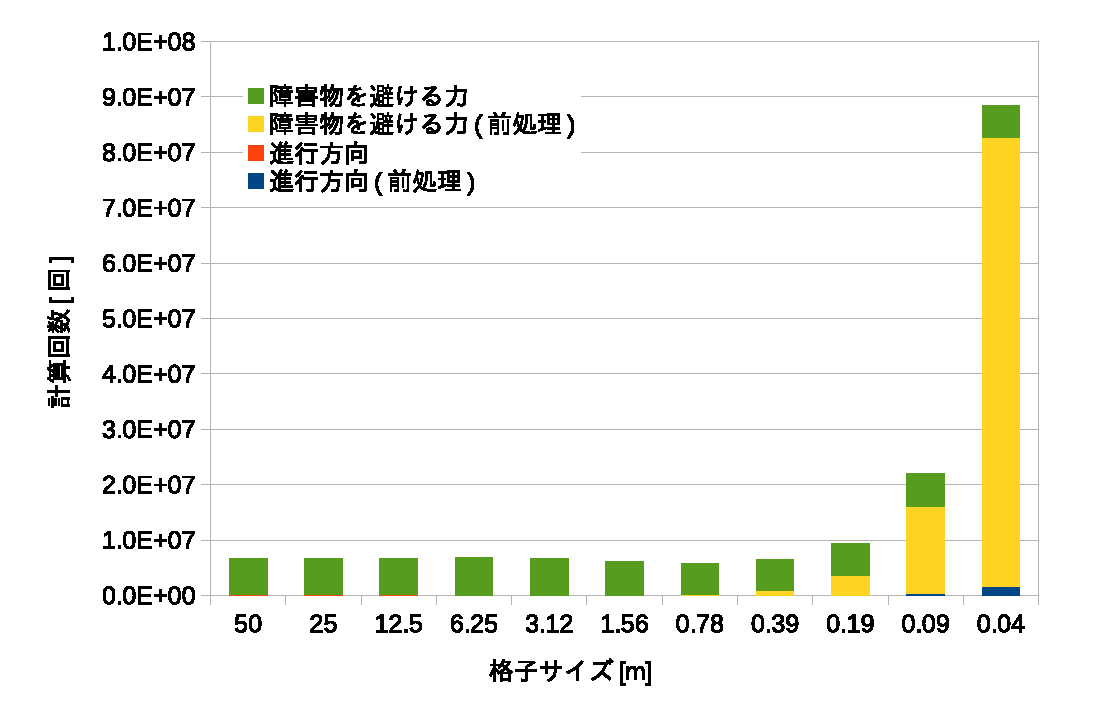
\includegraphics[width=\columnwidth]{figure/5_result_20m_times.eps}
		\caption{通路幅20mの格子サイズごとの計算回数}
		\label{fig:result_20m_times}
		\end{center}
	\end{minipage}
\end{figure}
%}}}

%削減率の表{{{
\begin{table}[tb]
  \centering
  \caption{各通路幅の格子サイズごとの計算回数の削減率[\%]}
  \label{tb:5_times_sakugenritu}
    \begin{tabular}{r|r|r|r|r}
    \hline \hline
              & 通路幅2m       & 通路幅5m       & 通路幅10m      & 通路幅20m     \\ \hline
        50.00 & 0.00           & 0.00           & 0.00           & 0.00          \\ \hline
        25.00 & 0.00           & 0.00           & 0.00           & 0.00          \\ \hline
        12.50 & 0.08           & 0.07           & 1.03           & 0.03          \\ \hline
        6.25  & 0.23           & 0.25           & -3.04          & -0.93         \\ \hline
        3.12  & 0.15           & 0.22           & -0.12          & 1.57          \\ \hline
        1.56  & 0.19           & 0.10           & 37.69          & 6.44          \\ \hline
        0.78  & 0.50           & 33.86          & \textbf{54.81} & \textbf{8.25} \\ \hline
        0.39  & \textbf{43.85} & \textbf{45.48} & 44.98          & 1.60          \\ \hline
        0.19  & 34.61          & 32.68          & 35.66          & -23.33        \\ \hline
        0.09  & -13.93         & -6.88          & -12.48         & -137.22       \\ \hline
        0.04  & -235.83        & -225.08        & -267.49        & -738.82       \\ \hline
    \end{tabular}
\end{table}
%}}}

\subsection{進行方向計算の計算回数}
\label{sec:5_calc_times}
本測定では,格子分割を用いた進行方向の計算回数削減手法の
有効性を評価するために,既存手法であるセル分割法と
格子分割を用いた進行方向の計算回数削減手法の計算回数を測定する.
測定する計算は,エージェントの進行方向の決定に必要な
エージェントの進行方向ベクトル$e$と
障害物を避ける力$F_{iW}$であり,前処理と解析中の回数である.
\figref{fig:result_2m_times},\figref{fig:result_5m_times},
\figref{fig:result_10m_times},\figref{fig:result_20m_times}に
各配置における計算回数を示す.
また,\tabref{tb:5_times_sakugenritu}に各配置における削減率を示す.
\tabref{tb:5_times_sakugenritu}に示す削減率は,式\eqref{eq:5_sakugenritu}
のように,セル分割法の各計算の総和$C_e$と提案手法の各計算の総和$C_p$を
用いて算出する.
%
\begin{eqnarray}
\mbox{削減率[\%]} = \Big ( 1 - \frac{C_p}{C_e}  \Big) \times 100
\label{eq:5_sakugenritu}
\end{eqnarray}
%

\figref{fig:result_2m_times}から\figref{fig:result_20m_times}より,
提案手法は,セル分割法よりも進行方向の計算回数が削減できる格子サイズが
あることが確認できる.
また,すべての配置において格子サイズが小さくなるほど,前処理の計算が
占める割合が高くなることがわかる.
これは,格子サイズが小さくなるほど,あらかじめ計算する進行方向を保持する
格子の要素数が多くなるため,前処理の計算回数が増えるためであると考えられる.
一方で,進行方向ベクトル$e$の計算は,各計算回数に対しての割合が低い.
これは,解析中の進行方向ベクトル$e$の計算回数が最大で
エージェント数とタイムステップ数の積であることから,障害物を避ける力の
計算回数よりも低いためであると考えられる.
%
\tabref{tb:5_times_sakugenritu}より,
提案手法がセル分割法に対して計算回数が削減できる格子サイズは,
通路幅2mで0.39mから0.19m,
通路幅5mで0.78mから0.19m,
通路幅10mで1.56mから0.19m,
通路幅20mで3.12mから0.78mであり,
通路幅が広くなるほど削減できる格子サイズの大きさが大きくなる.
これは,通路幅が広くなるほど,エージェントが通る場所の格子内に
壁粒子が含まれにくくなるため,あらかじめ計算した進行方向を
用いることができるからであると考えれれる.
[\textbf{炭治郎柄の図を使って説明しても良い}]
%
各通路幅の削減率は,\tabref{tb:5_times_sakugenritu}より,通路幅2mで最大43.85\%,
通路幅5mで最大45.48\%,通路幅10mで最大54.81\%,通路幅20mで最大8.25\%である.
通路幅20mの最大の削減率は,最大約8\%であり,他の通路幅の最大削減率(約50\%前後)と
比べて低いことがわかる.
これは,\figref{fig:result_2m_times}から\figref{fig:result_20m_times}より,
通路幅2mから10mのセル分割法の計算回数が約2000万回から約3000万回の間であるのに対して,
通路幅20mのときのセル分割法の計算回数が約500万回であり,
通路幅20mの計算回数が少なく,削減率が低くなったためであると考えられる.
また,
通路幅20mにおける既存手法の計算回数が少ない理由は,本評価で用いたパラメータの
影響範囲が5mであり,\figref{fig:haba20}に示すように,エージェントが通る場所が
通路幅20mであるため,エージェントの障害物を避ける力の影響範囲に壁粒子が存在しない
ことが多く,障害物を避ける力の計算回数が他の通路幅と比べて少ない結果が得られたと
考えられる.
%
\figref{fig:result_5m_times}から\figref{fig:result_20m_times}より,
前処理中の計算回数が占める割合は,どの通路幅の配置においても同様の傾向である結果が得られた.
これは,本評価に用いる配置の経由地数と解析領域が同じであるため,
式\eqref{eq:route_youso_size}や式\eqref{eq:fiw_youso_size}に示す前処理に必要な要素数が同じであり,
壁粒子数が同じであることから,通路幅が変わっても同様の傾向が得られたと考えられる.


%result figure {{{
\begin{figure}[tb]
	\begin{minipage}[b]{0.48\columnwidth}
		\begin{center}
		\includegraphics[width=\columnwidth]{figure/5_result_2bai_times.eps}
		\caption{通路幅2m(壁粒子2倍)の格子サイズごとの計算回数}
		\label{fig:result_2bai_times}
		\end{center}
	\end{minipage}
	\hspace{0.04\columnwidth}
	\begin{minipage}[b]{0.48\columnwidth}
		\begin{center}
		\includegraphics[width=\columnwidth]{figure/5_result_3bai_times.eps}
		\caption{通路幅2m(壁粒子3倍)の格子サイズごとの計算回数}
		\label{fig:result_3bai_times}
		\end{center}
	\end{minipage}
\end{figure}
%}}}
%昔の図{{{
%\figtb{通路幅2mの計算回数}{}{11}{5_result_2m_times.eps}{result_2m_times}
%\figtb{通路幅5mの計算回数}{}{11}{5_result_5m_times.eps}{result_5m_times}
%\figtb{通路幅10mの計算回数}{}{11}{5_result_10m_times.eps}{result_10m_times}
%\figtb{通路幅20mの計算回数}{}{11}{5_result_20m_times.eps}{result_20m_times}
%
%\figtb{通路幅2m(壁粒子2倍)の計算回数}{}{11}{5_result_2bai_times.eps}{result_2bai_times}
%\figtb{通路幅2m(壁粒子3倍)の計算回数(仮画像)}{}{11}{5_result_2bai_times.eps}{result_2bai_times}
%}}}
%削減率の表{{{
\begin{table}[tb]
  \centering
  \caption{各通路幅の格子サイズごとの計算回数の削減率[\%]}
  \label{tb:5_times_sakugenritu}
    \begin{tabular}{r|r|r|r|r}
    \hline \hline
              & 通路幅2m       & 通路幅5m       & 通路幅10m      & 通路幅20m     \\ \hline
        50.00 & 0.00           & 0.00           & 0.00           & 0.00          \\ \hline
        25.00 & 0.00           & 0.00           & 0.00           & 0.00          \\ \hline
        12.50 & 0.08           & 0.07           & 1.03           & 0.03          \\ \hline
        6.25  & 0.23           & 0.25           & -3.04          & -0.93         \\ \hline
        3.12  & 0.15           & 0.22           & -0.12          & 1.57          \\ \hline
        1.56  & 0.19           & 0.10           & 37.69          & 6.44          \\ \hline
        0.78  & 0.50           & 33.86          & \textbf{54.81} & \textbf{8.25} \\ \hline
        0.39  & \textbf{43.85} & \textbf{45.48} & 44.98          & 1.60          \\ \hline
        0.19  & 34.61          & 32.68          & 35.66          & -23.33        \\ \hline
        0.09  & -13.93         & -6.88          & -12.48         & -137.22       \\ \hline
        0.04  & -235.83        & -225.08        & -267.49        & -738.82       \\ \hline
    \end{tabular}
\end{table}
%}}}

%壁粒子数を変えたときの削減率{{{
\begin{table}[tb]
  \centering
  \caption{各通路幅の格子サイズごとの計算回数の削減率[\%]}
  \label{tb:5_bai_sakugenritu}
    \begin{tabular}{r|r|r|r}
    \hline \hline
		      & 壁粒子(1倍)    & 壁粒子(2倍)      & 壁粒子(3倍)        \\ \hline
		50.00 & 0.00           & 0.00             & 0.00               \\ \hline
		25.00 & 0.00           & 0.00             & 0.00               \\ \hline
		12.50 & 0.08           & 0.00             & 0.03               \\ \hline
		 6.25 & 0.23           & 0.03             & 0.08               \\ \hline
		 3.12 & 0.15           & 0.02             & 0.00               \\ \hline
		 1.56 & 0.19           & 0.05             & 0.11               \\ \hline
		 0.78 & 0.50           & 0.21             & 0.29               \\ \hline
		 0.39 & \textbf{43.85} & \textbf{47.00}   & \textbf{48.46}     \\ \hline
		 0.19 & 34.61          & 36.81            & 39.93              \\ \hline
		 0.09 & -13.93         & -14.68           & -13.39             \\ \hline
		 0.04 & -235.83        & -251.21          & -255.13            \\ \hline
    \end{tabular}
\end{table}
%}}}

\figref{fig:result_2bai_times},\figref{fig:result_3bai_times}より,
提案手法は,壁粒子数が増加した場合においても\figref{fig:result_2m_times}と同様に
格子サイズ0.39mから0.19mの間で削減できることが確認できる.
\figref{fig:result_2bai_times},\figref{fig:result_3bai_times}の結果から式\eqref{eq:5_sakugenritu}
を用いて算出した各配置の削減率を\tabref{tb:5_bai_sakugenritu}に示す.
\tabref{tb:5_bai_sakugenritu}中の太字の数値は,各配置の削減率の最大値を示す.
\tabref{tb:5_bai_sakugenritu}より,壁粒子数が多くなるほど,計算回数の削減率の最大値が高くなることがわかる.
これは,壁粒子の密度が高くなるほど,既存手法であるセル分割法の計算回数が増加するため,提案手法の
削減できる計算回数が多くなるためであると考えられる.

\clearpage
\subsection{シミュレーションの実行時間の測定}
\label{sec:5_calc_jikan}
\ref{sec:5_calc_times}節より,提案手法を用いることで,既存手法であるセル分割法よりも
進行方向の計算回数を削減できることが確認できた.
一方で,提案手法は,解析前にあらかじめ各格子の進行方向を計算するため,解析前の前処理の
実行時間は増加する.このため,あらかじめ計算するために必要な時間を考慮しても
格子分割を用いた進行方向の計算回数削減による高速化が有効であることを確認する.
\figref{fig:result_2m_jikan},\figref{fig:result_5m_jikan},
\figref{fig:result_10m_jikan},\figref{fig:result_20m_jikan}に通路幅ごとの
シミュレーション実行時間を,\figref{fig:5_kousokuka_haba}に式\eqref{eq:5_kousokuka}を用いて算出した
高速化率を示す.
また,\figref{fig:result_2bai_jikan},\figref{fig:result_3bai_jikan}に通路幅2mのときの
粒子数を2倍,3倍にした配置のシミュレーション実行時間を,\figref{fig:5_kousokuka_atusa}に高速化率を示す.
%
\begin{align}
	\mbox{高速化率[倍]} = \frac{\mbox{セル分割法の実行時間[s]}}
    {\mbox{提案手法の実行時間[s]}}
    \label{eq:5_kousokuka}
\end{align}
%
\figref{fig:result_2m_jikan},\figref{fig:result_5m_jikan},
\figref{fig:result_10m_jikan},\figref{fig:result_20m_jikan},
\figref{fig:5_kousokuka_haba}より,
提案手法は,セル分割法よりも最大△△倍高速であり,
従来手法よりも解析時間が最大○○割削減できることが確認できる.
また,格子サイズが小さくなるほど,前処理の計算にかかる時間の
割合が多くなり,通路幅2mでは0.09m,通路幅5mでは0.09m,通路幅10mでは
0.19m,通路幅20mでは0.39m以下の格子サイズで,従来手法よりも
遅くなることが確認できる.
前処理時間にかかる時間は,\ref{sec:5_calc_times}節で示した
前処理中の計算回数が占める割合の傾向と同様であることがわかる.
従来手法よりも高速に解析できる提案手法の格子サイズは,
通路幅2mで0.39mから0.19m,
通路幅5mで0.78mから0.19m,
通路幅10mで1.56mから0.19m,
通路幅20mで6.25mから0.39mであり,
通路幅が広くなるほど,従来手法よりも高速に解析できる格子サイズが
多くなることがわかる.
これをふまえると,従来手法よりも高速に解析できる提案手法の
格子サイズは,エージェントが通る場所の障害物と障害物の間の距離に
応じて変わることが考えられる.
\textbf{[壁粒子数を変えた時のシミュレーション実行時間と高速化率
について述べる!!!]} 

\figref{fig:result_2bai_jikan},\figref{fig:result_3bai_jikan},
\figref{fig:5_kousokuka_atusa}より,
提案手法のセル分割法に対する高速化率は,
壁粒子数1倍のときで最大○○倍,
壁粒子数2倍のときで最大○○倍,
壁粒子数3倍のときで最大○○倍であり,
壁粒子数が増えるほど高速化率の最大値が高くなることが確認できる.
これは,壁粒子を増やす方法が壁粒子の密度が高くなるような設定をしているため,
密度が高くなるほど,\ref{sec:5_calc_times}節で示した計算回数が削減でき,
解析時間の短縮に繋がったと考えられる.



\begin{figure}[tb]
	\begin{minipage}[b]{0.48\columnwidth}
		\begin{center}
		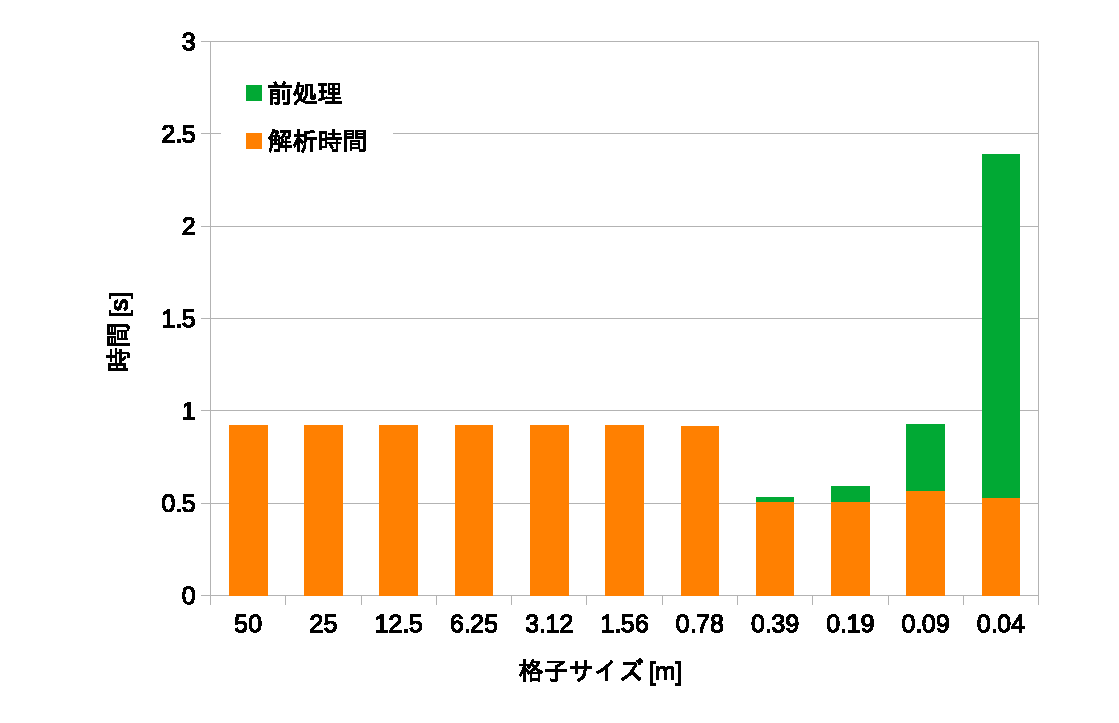
\includegraphics[width=\columnwidth]{figure/5_2m_jikan.eps}
		\caption{通路幅2mの格子サイズごとの解析時間}
		\label{fig:result_2m_jikan}
		\end{center}
	\end{minipage}
	\hspace{0.04\columnwidth}
	\begin{minipage}[b]{0.48\columnwidth}
		\begin{center}
		\includegraphics[width=\columnwidth]{figure/5_5m_jikan.eps}
		\caption{通路幅5mの格子サイズごとの解析時間}
		\label{fig:result_5m_jikan}
		\end{center}
	\end{minipage}
\end{figure}

\begin{figure}[tb]
	\begin{minipage}[b]{0.48\columnwidth}
		\begin{center}
		\includegraphics[width=\columnwidth]{figure/5_10m_jikan.eps}
		\caption{通路幅10mの格子サイズごとの解析時間}
		\label{fig:result_10m_jikan}
		\end{center}
	\end{minipage}
	\hspace{0.04\columnwidth}
	\begin{minipage}[b]{0.48\columnwidth}
		\begin{center}
		\includegraphics[width=\columnwidth]{figure/5_20m_jikan.eps}
		\caption{通路幅20mの格子サイズごとの解析時間}
		\label{fig:result_20m_jikan}
		\end{center}
	\end{minipage}
\end{figure}

\begin{figure}[tb]
	\begin{minipage}[b]{0.48\columnwidth}
		\begin{center}
		\includegraphics[width=\columnwidth]{figure/5_2bai_jikan.eps}
		\caption{通路幅2m(粒子数2倍)の格子サイズごとの解析時間}
		\label{fig:result_2bai_jikan}
		\end{center}
	\end{minipage}
	\hspace{0.04\columnwidth}
	\begin{minipage}[b]{0.48\columnwidth}
		\begin{center}
		\includegraphics[width=\columnwidth]{figure/5_3bai_jikan.eps}
		\caption{通路幅3m(粒子数3倍)の格子サイズごとの解析時間}
		\label{fig:result_3bai_jikan}
		\end{center}
	\end{minipage}
\end{figure}


\begin{figure}[tb]
 \begin{center}
  \includegraphics[width=12.5cm,clip]{figure/5_kousokukaritu.eps}
  \caption{通路幅を変えたときの高速化率}
  \label{fig:5_kousokuka_haba}
 \end{center}
\end{figure}


\begin{figure}[tb]
 \begin{center}
  \includegraphics[width=12.5cm,clip]{figure/5_bai_kousokukaritu.eps}
  \caption{壁粒子数を変えたときの高速化率}
  \label{fig:5_kousokuka_atusa}
 \end{center}
\end{figure}

\if 0
\clearpage
\subsection{シミュレーション精度の測定}
\ref{sec:5_calc_jikan}節より,
提案手法は,一部の格子サイズでセル分割法よりも高速に解析できることが確認できた.
一方で,本手法は,解析領域を格子状に分割した格子ごとに計算した進行方向ベクトル$e$と
障害物を避ける力$F_{iW}$を解析中に用いるため,セル分割法のシミュレーションと比べて
シミュレーション誤差が生じる手法となる.
このため,提案手法の格子ごとのシミュレーション結果と従来手法であるセル分割法の
シミュレーション結果を比較し,シミュレーション精度を確かめる.
誤差は,提案手法とセル分割法が算出した時間ステップごとに各エージェントの座標を
出力し,2手法の同時刻・同エージェントどうしによるエージェント間距離である.

\textbf{
[図○○に各配置のシミュレーションの最大誤差を示す.]
}
\fi

\clearpage
%配置のイメージ図{{{
\begin{figure}[tb]
	\begin{minipage}[b]{0.5\columnwidth}
		\centering
		\includegraphics[width=\columnwidth]{figure/kyositu_v2.eps}
		\caption{教室の初期配置}
    \label{fig:kyositu_haichi}
	\end{minipage}
	\begin{minipage}[b]{0.5\columnwidth}
		\centering
		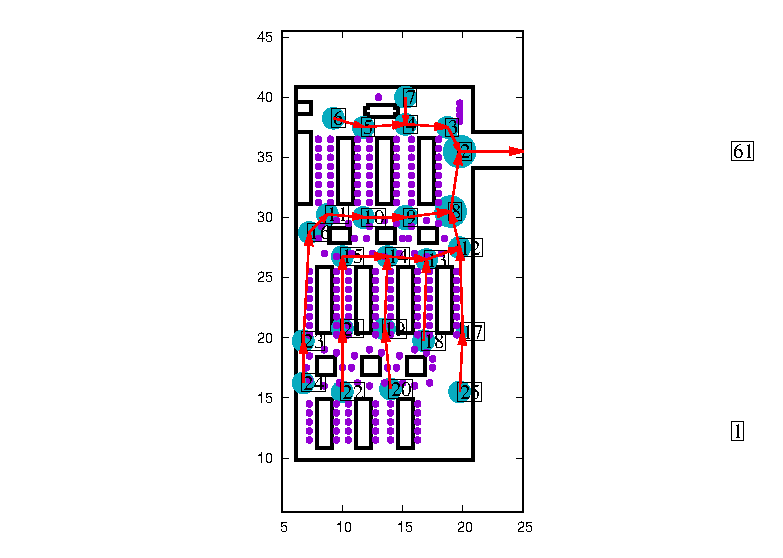
\includegraphics[width=\columnwidth]{figure/pc_m.eps}
		\caption{演習室の初期配置}
    \label{fig:pc_haichi}
	\end{minipage}
\end{figure}
%}}}
%各配置における粒子数{{{
\begin{table}[tb]
  \begin{center}
    \caption{各配置の詳細}
    \label{tb:haichi_para}
    \begin{tabular}{c|c|c}
      \hline \hline
      & 教室 & 演習室 \\ \hline 
      エージェント数[人] & 96 & 204 \\ \hline
      壁粒子数[個] & 1037 & 1454\\ \hline
      経由地数[個] & 12   & 26 \\ \hline
      解析領域 & $50m\times50m$ & $50m\times50m$ \\ \hline
    \end{tabular}
  \end{center}
\end{table}
%}}}
\subsection{避難シミュレーションに対する提案手法の有効性}
\label{sec:5_real}
本節では,実問題に対する提案手法の有効性を示すために,実際の状況下で
避難シミュレーションを行い,シミュレーション実行時間とシミュレーション精度を
確かめる.
本評価に用いるエージェントの初期配置は,\figref{fig:kyositu_haichi},\figref{fig:pc_haichi}に示すように,大学の演習室や教室の避難時の配置で設定する.
\figref{fig:kyositu_haichi},\figref{fig:pc_haichi}の黒点は壁粒子,紫色の点はエージェント,青色の丸は経由地の座標およびゴール判定の大きさ,赤色の矢印は経由地のグラフを示す.
それぞれの配置のエージェントや壁,経由地は,\tabref{tb:haichi_para}に示すような数で配置する.
本測定では,パラメータを\tabref{tb:result_para}で設定し,すべてのエージェントが
部屋から避難できるまでを刻み値0.001で解析する.
\figref{fig:kyositu_time}に教室を再現した配置の格子サイズごとのシミュレーション実行時間を,
\figref{fig:pc_time}に演習室を再現した配置の格子サイズごとのシミュレーション実行時間を示す.

\figref{fig:kyositu_time},\figref{fig:pc_time}より,
セル分割法のシミュレーション実行時間は,
教室を再現した配置で\textbf{6.0秒},
演習室を再現した配置で\textbf{24.5秒}である.
また,提案手法のシミュレーション実行時間は,
格子サイズ0.19mのとき,
教室を再現した配置で\textbf{3.5秒},
演習室を再現した配置で\textbf{15.5秒}である.
提案手法の高速化率は,教室を再現した配置で最大1.6倍,
演習室を再現した配置で最大1.5倍である.
このため,提案手法は避難シミュレーションにおいても,
セル分割法よりも高速に解析できることがわかる.
%配置で高速化率が違う理由について考察したい.

%教室と演習室の解析時間{{{
\begin{figure}[tb]
	\begin{minipage}[b]{0.48\columnwidth}
		\begin{center}
		\includegraphics[width=\columnwidth]{figure/20231016_kyositu_time.eps}
		\caption{教室の配置における格子サイズごとの解析時間}
		\label{fig:kyositu_time}
		\end{center}
	\end{minipage}
	\hspace{0.04\columnwidth}
	\begin{minipage}[b]{0.48\columnwidth}
		\begin{center}
		\includegraphics[width=\columnwidth]{figure/20231016_pc_time.eps}
		\caption{演習室の配置における格子サイズごとの解析時間}
		\label{fig:pc_time}
		\end{center}
	\end{minipage}
\end{figure}
%}}}
%
%教室と演習室の誤差{{{
\begin{figure}[tb]
	\begin{minipage}[b]{0.48\columnwidth}
		\begin{center}
		\includegraphics[width=\columnwidth]{figure/20231016_kyositu_gosa.eps}
		\caption{教室の配置における格子サイズごとの最大誤差}
		\label{fig:kyositu_gosa}
		\end{center}
	\end{minipage}
	\hspace{0.04\columnwidth}
	\begin{minipage}[b]{0.48\columnwidth}
		\begin{center}
		\includegraphics[width=\columnwidth]{figure/20231016_pc_gosa.eps}
		\caption{演習室の配置における格子サイズごとの最大誤差}
		\label{fig:pc_gosa}
		\end{center}
	\end{minipage}
\end{figure}
%}}}
%
本測定の精度は,エージェントの座標誤差と,
避難完了時間の誤差を用いて評価する.
エージェントの座標誤差は,提案手法とセル分割法が算出した時間ステップごとに各エージェントの座標を
出力し,2手法の同時刻・同エージェントどうしによるエージェント間距離である.
また,避難完了時間の誤差は,セル分割法と提案手法が解析した
避難を完了した時間を出力し,\eqref{eq:gosa_hinan}を用いて算出する.
%
\begin{eqnarray}
\label{eq:gosa_hinan}
\mbox{避難完了時間の誤差$[\%]$} = \left | \frac{C_{time} - T_{time}}{C_{time}} \right | \times 100
\end{eqnarray}
%
\eqref{eq:gosa_hinan}中の$C_{time}$はセル分割法の避難完了時間であり,
$T_{time}$は提案手法の避難完了時間である.
\figref{fig:kyositu_gosa}に教室を再現した配置の格子サイズごとの座標誤差,
\figref{fig:pc_gosa}に演習室を再現した配置の格子サイズごとの座標誤差を示す.
\figref{fig:kyositu_gosa},\figref{fig:pc_gosa}より,
本測定条件下の提案手法の座標誤差は,
教室を再現した配置で最大\textbf{2.6cm},
演習室を再現した配置で最大\textbf{2.6cm}である.
両方の配置で誤差が横ばいである理由は,目的地や障害物が含まれる格子では,
進行方向を簡易化せずにエージェントごとに個別で計算しているため,格子サイズが
大きくなるほど生じる誤差を抑えることができたためであると考えられる.
また,提案手法の生じる誤差は,両方の配置で解析領域が$50m\times50m$,人の大きさが
$0.25m$であることを踏まえると小さな値であり,実用的であると考えられる.
本測定条件下のセル分割法の避難完了時間は,
教室を再現した配置で\textbf{○○秒},
演習室を再現した配置で\textbf{○○秒}である.
また,本測定条件下の格子サイズ$0.19m$の提案手法の避難完了時間は,
教室を再現した配置で\textbf{○○秒},
演習室を再現した配置で\textbf{○○秒}である.
本測定条件下の提案手法の避難完了時間の誤差は,
教室を再現した配置で\textbf{○○\%},
演習室を再現した配置で\textbf{○○\%}である.
この誤差は,関連研究\cite{???}\textbf{[一次元化の参考文献]}と比較すると
小さな値であり,提案手法が避難シミュレーションにおいても実用的な誤差であることがわかる.


%\figtb{格子サイズごとの解析時間(教室)}{}{10}{20231016_kyositu_time}{kyositu_time}
%\figtb{格子サイズごとの解析時間(演習室)}{}{10}{20231016_pc_time.eps}{pc_time}
%\figtb{格子サイズごとの最大誤差(教室)}{}{9}{20231016_kyositu_gosa}{kyositu_gosa}
%\figtb{格子サイズごとの最大誤差(演習室)}{}{9}{20231016_pc_gosa.eps}{kyositu_gosa}
\section{本章のまとめ}
本章では,SFMを用いた人流シミュレーションを高速化するために,
格子分割を用いた進行方向の計算回数を削減する手法を提案し,その有効性を評価した.
評価の結果,提案手法は,通路を再現した配置を移動する問題において,
エージェントの進行方向の計算回数を最大○○\%削減し,シミュレーション実行時間を
最大○○倍高速に解析できることを確認した.
また,提案手法は,避難シミュレーションにおいても,大学の施設を再現した配置から避難する様子を
再現する解析で十分に許容できる誤差の範囲で最大○○倍高速に解析できることを確認した.


% vim: set tabstop=4 :
%**********************************************************
\chapter{おわりに}
\label{sec:discuss}
%**********************************************************
本論文では,これまで述べてきた提案手法とその評価結果をまとめ,本研究全体の総括を行う.
本研究では,SFMを用いた人流シミュレーションを高速化するために,
エージェント間距離の計算回数削減手法と,
進行方向の計算回数削減手法を提案し,その有効性を評価した.

第\ref{sec:reduce_distance}章「エージェント間距離の計算回数削減手法」では,
視野パラメータを用いたSFMの人流シミュレーションにおいて,周囲のエージェントが
視野範囲内に存在するかの判定に必要なエージェント間距離の計算回数を削減する手法を提案した.
SFMを用いた人流シミュレーションは,一般的にセル分割法を用いることで,
エージェント間距離の計算回数の削減が行われている.
セル分割法は,影響範囲が円形であることを前提としており,視野を用いたSFMのように影響範囲が
扇形の場合を想定していない.
このため,視野を用いたSFMに一般的なSFMのエージェント間距離の計算回数削減手法を用いると,
影響範囲を円形に絞り込みをした上で,視野形状に合わせた扇形に絞り込みを行う操作が必要となる.
本提案手法では,視野形状である扇形に近似した領域を設定し,
近似領域外のエージェントに対するエージェント間距離の計算回数を削減することで,
視野を用いたSFMを高速化する.
評価の結果,提案手法は,エージェントが交差するように移動する問題において,
十分に許容可能な誤差の範囲で約1.25倍の高速化率が得られることを確認した.
%他にもあればここに追記予定


第\ref{sec:reduce_travel_direction}章「格子分割を用いた進行方向の計算回数削減手法」では,
SFMを用いた人流シミュレーションにおいて,
進行方向をあらかじめ計算することで,解析中の進行方向の計算回数を削減する手法を提案した.
本手法は,目的地や障害物の座標が解析中に変化しない特徴を利用し,解析領域を格子状に分割した
領域ごとに目的地に向かうベクトルと障害物を避ける力を計算し,解析中にその値を用いて
解析する
評価の結果,提案手法は,通路を再現した配置を移動する問題において,
エージェントの進行方向の計算回数を最大○○\%削減し,シミュレーション実行時間を
最大○○倍高速に解析できることを確認した.
また,提案手法は,避難シミュレーションにおいても,大学の施設を再現した配置から避難する様子を
再現する解析で十分に許容できる誤差の範囲で最大○○倍高速に解析できることを確認した.

以上の結果より,SFMを用いた人流シミュレーションにおいて,ふたつの手法で計算回数を削減し,
高速化を確認した.第\ref{sec:reduce_distance}章で提案した手法は,視野パラメータを用いた
SFM

\textbf{続く}


%***** END ************************************************


%------------------------------------------------------------------
% 注意点
%------------------------------------------------------------------
% 「おわりに」は,ここまでの文章をすべて読んできた人向けの文章です.
% このため,細かな用語の説明は必要ありません.
% 論文の論理構造が分かるような文章を1\UTF{FF5E}2ページ目安で書いてください.
% 
% 構成例を以下に示します.
% [1段落目]
% 従来手法の問題点とそれに対する提案手法
% [2段落目]
% 提案手法の手順
% [3]段落目以降
% 評価結果とそこから導き出される結論
%
%------------------------------------------------------------------



%====[ 謝辞 ]========================================================
\clearpage
\addcontentsline{toc}{chapter}{謝辞}
\markright{謝辞}
% vim: set tabstop=4 :
%******************************************************************
\chapter*{謝辞}
\label{sec:thanks}
%******************************************************************
aa
aa




\thanksend
%************************* END ************************************


%------------------------------------------------------------------
% 謝辞例文集(これが礼儀的にどうなのかは謎.自己責任で使用すること)
%               ※指導教員の名前は必ず書くのが礼儀です.
%------------------------------------------------------------------
%
% 本研究の機会及び素晴らしい実験環境を与えて下さり,
% 貴重な時間を割いて研究の方向性を御指導頂きました○○ ○○教授に
% 深く感謝致します.
%
% 本研究を進めるにあたり,
% 日頃から惜しみなく御指導して頂きました○○ ○○氏に
% 心から感謝致します.
%
% 研究の方向性をはじめ研究の細部に至るまで数々の有意義な御意見,
% 御助言を賜わりました○○ ○○氏に
% 感謝致します.
%
% 特に,本研究のきっかけを与えて下さり,研究の進め方から文章の
% 書き方まで丁寧に御指導下さった
% ○○ ○○氏には
% この場を借りて心から深く感謝致します.
%
% 貴重な御意見,様々な御提案を頂いた××ゼミの皆様に御礼申し上げます.
%
% 最後に,私をここまで育てて下さった家族に深く感謝します.
%
%------------------------------------------------------------------


%====[ 参考文献 ]====================================================

\clearpage
\addcontentsline{toc}{chapter}{参考文献}
\markright{参考文献}
\bibliography{bibfile1}          % どちらか片方を選択     
%%ここに参考文献を入力

\begin{thebibliography}{99}
\bibitem{soturon1}
	  aaaaaaaaaaaaaaaaa
  \bibitem{soturon2}
	 虞飛,佐藤裕幸: aa高解像度画像対応ステレオマッチングのGPGPUによる
	  高速化,情報処理学会研究報告,Vol.2017-HPC-160 No.19 (2017).
  \bibitem{soturon3}
	  大田弘樹,馬場明子,下田雄一,安田隆洋,山本啓二: GPGPUを用い
	  たソフトウェア高速化手法,MSS技報,Vol27 (2017).
  \bibitem{soturon4}
	  Hisa Ando:GPUを支える技術,技術評論社(2017)
  \bibitem{soturon5}
	  柳田匠,田中輝雄,藤井昭宏: GPUを用いた行列-行列積の実装と性能
	  評価,情報処理学会第81回全国大会,(2019)
  \bibitem{soturon6}
	  K.F.RILEY,M.P.HOBSON,and S.J.BENCE:Mathematical Methods for
	  physics and engineering,Cambridge University Press(2010).
  \bibitem{soturon7}
	  Cheng.J,Grossman.M,and McKercher.T.株式会社クイープ:CUDA C
	  プロフェッショナルプログラミング,インプレス(2015).
  \bibitem{soturon8}
	  NVIDIA TESLA V100 GPU ARCHITECTURE, available from<http://images.
nvidia .com/content/volta-architecture/pdf/volta-architecture-whitepaper.pdf>
	  (accessed 2020-11-16).
  \bibitem{soturon9}
	  Dissecting the NVIDIA Volta GPU Architecture via
	  Microbenchmarking,available
	  from<https://arxiv.org/pdf/1804.06826.pdf>(accessed
	  2020-11-25)
  \bibitem{soturon10}
	  Using Tensor Cores for Mixed-Precision scientific Computing,
	  available
	  from<https://developer.nvidia.com/blog/tensor-cores-mixed-precision-scientific-com
	  puting>(accessed 2020-11-20)
  \bibitem{soturon11}
	  Programming Tensor Cores in CUDA9,available
	  from<https://developer.nvidia.com/blog/programming-tensor-cores-cuda-9/>(accessed
	  2020-11-25)
	  
 \bibitem{soturonaaaaaaaa}	 
	 Kerr,A.Merril,D.Demouth,J.Tran,J:CUTLASS:Fast Linear
	 Algebra in CUDA C++,NVIDIA Developer Blog(オンライン),
	 available
	 from<https://developer.nvidia.com/blog/cutlass-linear-algebra
	 -cuda>(accessed2020-09-02).
	 
%人名,人名:研究タイトル,書籍名,Vol.数値,No.数値,pp.数値-数値(発行年).
\end{thebibliography}
                        % どちらか片方を選択


%====[ 付録 ]========================================================
\appendixes             %付録に章番号が必要ない場合は"es"を削除(\appendixにする)
% vim: set tabstop=4 :
%**********************************************************
\chapter{プログラムの説明}
\label{sec:appendix}
%**********************************************************
付録には,添付するソースコードの説明を書いてください.
データ構造や主要な変数の説明は本文中で述べてあると思います.
本文で述べたことを一覧形式でまとめる分には構いませんが,
まったく同じことを書くのはよくありません.
このため,本文中では書けない実装の話
(コンパイル方法や, 測定条件の変更方法,入出力フォーマットなど)
を中心に書きましょう.

また,付録のページは,
本文中で邪魔になった定義とか証明とかの避難場所としても利用可能です.

\section{データ構造}
エージェントのデータ構造は,agent\_tの構造体名で構造体配列として
保持する.agent\_tの構造体中のメンバを下記に示す.
%
\begin{itembox}[l]{エージェントの構造体}
typedef struct\{\\
 int num;\\
 double x, y;\\
 double gx, gy;\\
 int r\_num;\\
 struct route\_t *goal\_p;\\
\}agent\_t;
\end{itembox}
%
agent\_t中のnumのメンバはエージェントの番号,xとyのメンバはエージェント
の座標,gxとgyのメンバは目的地の座標,r\_numのメンバは経由地の番号,
*goal\_pのメンバはエージェントが向かう経由地のポインタを示す.
経由地のデータ構造造は,route\_tの構造体名で構造体配列として
保持する.route\_tの構造体中のメンバを下記に示す.
%
\begin{itembox}[l]{経由地の構造体}
typedef struct\{\\
 int num;\\
 double x, y;\\
 double rad:\\
 int next\_num;\\
 struct route\_t *next;\\
 double **ex, **ey;\\
\}route\_t;
\end{itembox}
%
route\_t中のnumのメンバは経由地の番号,xとyのメンバは経由地の座標,
radのメンバは経由地のゴール判定の半径,next\_numのメンバは,
次の経由地番号,*nextのメンバは次の経由地のポインタ,
**exと**eyのメンバは,格子分割を用いた場合の前処理で算出した
経由地までの進行方向を保持する配列である.

壁粒子のデータ構造は,wall\_tの構造体名で単方向リストとして
保持する.本論文は,壁を複数の粒子として実装しているため,
壁粒子から受ける力の計算にセル分割法を用いる.
壁粒子は,解析開始から終了まで固定されているため,座標が変化しない.
このため,壁粒子のセル分割法のデータ構造は,シミュレーション開始の
一回のみの生成となるため,連結リスト法で実装する.
下記に壁粒子の構造体を示す.
%
\begin{itembox}[l]{壁粒子の構造体}
typedef struct \{\\
 double x, y;\\
 struct wall\_t *np;\\ 
\}wall\_t;
\end{itembox}
%
wall\_t中のxとyのメンバは壁粒子の座標,*npのメンバは次の壁粒子の
ポインタを示す.
下記にエージェントのセル分割法に用いるハッシュ法の構造体cell\_tの
メンバを示す.
\begin{itembox}[l]{セル分割法(ハッシュ法)の構造体}
typedef struct \{\\
 int *hash;\\
 int *index;\\
 int *start;\\
\}cell\_t;
\end{itembox}
構造体cell\_t中の*hashのメンバはハッシュ法のハッシュ配列,*indexのメンバはハッシュ法の
インデックス配列,*startのメンバはハッシュ法のスタート配列である.
エージェントのセル分割法は,時間ステップごとにエージェントの座標が変わるため,
時間ステップごとに再構築する必要がある.このため,再構築する速度や
保守性の観点からセル分割法の中でもハッシュ法を構造体としてデータを保持する.

\section{プログラムのファイル構造}
SFMを用いた人流シミュレーションのファイル構造を下記に示す.
%
\begin{itembox}[l]{プログラムのファイル構造}
  \dirtree{%
  .1 \includegraphics[width=0.25cm]{dire.png} sfm\_program.
  .2 sfm.c.
  .2 \includegraphics[width=0.25cm]{dire.png} inputwall.
  .3 pc\_3.c.
  .3 kyositu.c.
  }
\end{itembox}
%
sfm.cは,SFMを用いた人流シミュレーションのプログラムであり,C言語で記述されている.
inputwall内に存在するC言語のファイルは,sfm.cで用いるエージェントや壁,経由地の初期
配置が記述されたコードである.
\tabref{tb:arrangement_gimp_files}に本論文中の評価で使用した初期配置のファイル名
を示す.
\tabref{tb:arrangement_gimp_files}に示すファイルは,sfm.c中にインクルードすることで
使用することができる.

\begin{table}[H]
  \begin{center}
    \caption{本論文中の評価で使用した初期配置}
    %\ecaption{The evaluation environment.}
    \label{tb:arrangement_gimp_files}
    \begin{tabular}{c|c}
      \hline \hline
      配置名 & ファイル名 \\ \hline
      演習室 & pc\_3.c \\ \hline
      教室 & kyositu.c \\ \hline
      演習室(dense) & pc\_3\_dense.c \\ \hline
      演習室(sparse) & pc\_3\_sparse.c \\ \hline
      演習室(sparse\&wide) & pc\_3\_sparse\_wide.c \\ \hline
      通路(幅2m) & haba2.c \\ \hline
    \end{tabular}
  \end{center}
\end{table}


\section{実行方法}
SFMを実装したプログラムのコンパイルは下記のコマンドの通りである.
\begin{itembox}[l]{コンパイル方法}
  gcc [ファイル名] -lm -O3 `pkg-config --cflags --libs glib-2.0`
\end{itembox}
本プログラムの入力データは,GIMPを用いてC言語に出力したものであり,
プログラム上で処理するためにglib.hをインクルードする必要がある.
glib.hをインクルードするためには,コンパイル時に`pkg-config --cflags --libs glib-2.0`を
追記することが必要である.

コンパイルして生成されたファイルは,次のコマンドで実行することができる.
\begin{itembox}[l]{実行方法}
./[実行ファイル名] [実行ステップ数] [格子サイズ]
\end{itembox}
第2引数は,実行ステップ数で解析したいステップ数を入力する必要がある.
第3引数は,提案手法の格子サイズを入力する必要がある.既存手法で実行する
場合は,第3引数を使うことがないが仮に入力が求められる.
既存のセル分割法と提案手法は.一つのファイルで構成されており,
切り替えるために,\#DEFINEで定義された変数(KIZON)が使用されている.
\tabref{tb:toggle_kizon}に既存手法と提案手法を切り替えるための
変数(KIZON)の状態を示す.
%
\begin{table}[H]
  \begin{center}
    \caption{既存手法と提案手法の切り替え方法}
    %\ecaption{The evaluation environment.}
    \label{tb:toggle_kizon}
    \begin{tabular}{c|c}
      \hline \hline
      \#DEFINE KIZON     & 既存手法(セル分割法)で実行 \\ \hline
      //\#DEFINE KIZON & 格子分割を用いた進行方向計算の削減手法で実行\\ \hline
    \end{tabular}
  \end{center}
\end{table}
%
\tabref{tb:toggle_kizon}に示すように,提案手法で実行する場合は,
\#DEFINE KIZONをコメントアウトする必要がある.

\section{測定条件の変更方法}
本節では,測定条件のパラメータの変更方法について述べる.
測定条件のパラメータは,C言語中の\#DEFINEを用いた変数で設定できる.
\tabref{tb:parameter_settings}にそれぞれの変数とパラメータ内容に
ついて示す.\tabref{tb:parameter_settings}中のパラメータの初期設定
は,\tabref{tb:tab_para}と同じ値である.


%tb:定数設定
\begin{table}[t]
  \begin{center}
    \caption{測定条件のパラメータ変数}
    \label{tb:parameter_settings}
    \begin{tabular}{c|c}
      \hline \hline
      変数名 & 内容 \\ \hline
      A\_I & $A_i$ \\ \hline
      B\_I & $B_i$ \\ \hline 
      K   & $k$   \\ \hline 
      KAPPA & $\kappa$  \\ \hline 
      V\_0 & $v_i^0$     \\ \hline 
      M\_I & $m_i$       \\ \hline 
      TAU & $\tau_i$    \\ \hline 
      R\_I & $r_i$       \\ \hline 
      H   & 刻み値 \\ \hline
      MAX\_SPEED & 最大歩行速度 \\ \hline
      NEIGHBOR\_RADIUS & エージェントの影響半径 \\ \hline

    \end{tabular}
  \end{center}
\end{table}

\section{初期配置のデータの生成方法}


\begin{table}[H]
  \begin{center}
    \caption{動作確認済み環境}
    %\ecaption{The evaluation environment.}
    \label{tb:conform_env}
    \begin{tabular}{c|c}
      \hline \hline
      CPU              & Intel Xeon CPU E5-2687w v2 \\ \hline
      メモリ           & 16GB                       \\ \hline
      OS               & Linux 4.12.9               \\ \hline
      GIMPバージョン & x.x.x \\ \hline
    \end{tabular}
  \end{center}
\end{table}


\begin{figure}[H]
  \begin{center}
    \includegraphics[width=5cm,clip]{figure/gimp1.png}
    \caption{GIMPの出力ファイル形式の選択}
    \label{fig:gimp1}
  \end{center}
\end{figure}


\begin{figure}[H]
  \begin{center}
    \includegraphics[width=5cm,clip]{figure/gimp2.png}
    \caption{GIMPのC言語出力画面}
    \label{fig:gimp1}
  \end{center}
\end{figure}


\section{節番号のテスト}
\subsection{項番号のテスト}
付録では,こんな風に章番号が表示されます.
付録A, 付録Bというように,付録のchapterにも章番号をつけたい場合は,
main.tex66行目の$\setminus$appendixを$\setminus$appendixesに変更してください.


%***** END ************************************************

\end{document}
